\documentclass[12pt,twoside]{article}
\usepackage[dvipsnames]{xcolor}
\usepackage{tikz,graphicx,amsmath,amsfonts,amscd,amssymb,bm,cite,epsfig,epsf,url}
\usepackage[hang,flushmargin]{footmisc}
\usepackage[colorlinks=true,urlcolor=blue,citecolor=blue]{hyperref}
\usepackage{amsthm,multirow,wasysym,appendix}
\usepackage{array,subcaption} 
% \usepackage[small,bf]{caption}
\usepackage{bbm}
\usepackage{pgfplots}
\usetikzlibrary{spy}
\usepgfplotslibrary{external}
\usepgfplotslibrary{fillbetween}
\usetikzlibrary{arrows,automata}
\usepackage{thmtools}
\usepackage{blkarray} 
\usepackage{textcomp}
\usepackage[left=0.8in,right=1.0in,top=1.0in,bottom=1.0in]{geometry}

\begin{document}

\begin{center}
{\large{\textbf{Homework 4}} } \vspace{0.2cm}\\
Due October 10 at 11 pm
\\
\end{center}


\begin{enumerate}

\item (Halloween) In Halloween Laura and her brother Mike arrive at a house where they offer them a bowl with 2 chocolate bars. Mike grabs a random number of chocolate bars; he grabs 0, 1, or 2 with the same probability. Laura then grabs some chocolate bars out of the remaining ones; also with uniform probability (there is the same probability that she grabs 0, 1, etc.).
\begin{enumerate}
\item Model the number of bars grabbed by Mike and the number of bars grabbed by Laura as random variables and compute their joint pmf.
\subitem 
We can represent the joint pmf by creating a matrix table who's entries represents the probabilities of all possibilities. Each number under Laura or Mike's name represents the amount of chocolate bars they have after they each have a turn grabbing bars from the bowl. The intersection of each number is the probability of the joint pmf for the occurrence of both events. 
$$
    \text{Mike}
    \begin{pmatrix}
    \ & \ & \text{Laura} & \ \\
    \ & 0 & 1 & 2 \\
    0 & 1/9 & 1/9 & 1/9 \\
    1 & 1/6 & 1/6 & 0 \\
    2 & 1/3 & 0 & 0
    \end{pmatrix}
$$

\item Compute the marginal pmf of the number of bars grabbed by Laura. 
\subitem We can compute the marginal pmf of any number of bars grabbed by Laura by summing each row:
$$
    P(\Tilde{L}=0) = \frac{11}{18} \  P(\Tilde{L}=1) = \frac{5}{18} \ P(\Tilde{L}=2) = \frac{2}{18}
$$
\item What is the conditional pmf of the number of bars grabbed by Mike if we know that Laura grabbed 1 bar?
\subitem Knowing that Laura has 1 bar we can readjust Mike's probabilities. We can do so, by normalizing each entry in the column that corresponds to the event that Laura has taken 1 bar.
$$
    P(\Tilde{M}=0) = \frac{\frac{2}{18}}{\frac{5}{18}} = \frac{2}{5} \  P(\Tilde{M}=1) = \frac{\frac{3}{18}}{\frac{5}{18}} = \frac{3}{5} \ P(\Tilde{M}=2) = \frac{0}{\frac{5}{18}} = 0
$$
We can see that since Laura has 1 chocolate bar, it completely eliminates the possibility that Mike has two bars. The only possibilities, that Mike has 0 or 1 bars of chocolate, get increased to $\frac{2}{5}$ and $\frac{3}{5}$ respectively when we normalize our probability space such that the event that Mike has 0 or 1 bar of chocolate is 100$\%$.
\end{enumerate}

\break

\item (Interview)
A company is interviewing candidates for a data-scientist position. They estimate that the probability of a candidate being well qualified is 0.25. This is modeled by a random variable $\Tilde{Q}$ that equals 1 with probability 0.25, and -1 with probability 0.75. Candidates are interviewed separately by two interviewers. The decision of the interviewers are modeled as two random variables $\Tilde{i}_1 = \Tilde{e}_1\Tilde{Q}$ and $\Tilde{i}_2 = \Tilde{e}_2\Tilde{Q}$, where $\Tilde{e}_1$ and $\Tilde{e}_2$ are random variables that model the probability that the interviewers make a mistake. They both equal 1 with probability 0.8 (no mistake) and -1 with probability 0.2 (mistake). $\Tilde{e}_1$, $\Tilde{e}_2$, and $\Tilde{Q}$ are all mutually independent.      
\begin{enumerate}
\item What is the probability that the outcome of both interviews is positive, i.e. that $\Tilde{i}_1=1$ and $\Tilde{i}_2=1$? 
\subitem
We can calculate this outcome, since $\Tilde{e}_1$, $\Tilde{e}_2$, and $\Tilde{Q}$ are all mutually independent. There are only two cases where both interviews are positive, when both interviews have the correct judgement on a correct candidate ($\Tilde{e}_1=1, \Tilde{e}_2=1, \Tilde{q}=1$), and when both interviewers make mistakes on an unqualified candidate: ($\Tilde{e}_1=-1, \Tilde{e}_2=-1, \Tilde{q}=-1$). We can add these probabilities to find the total:
\begin{equation}
    \begin{split}
       P(\Tilde{e}_1=1, \Tilde{e}_2=1, \Tilde{q}=1) = .8*.8*.2 = .16 
    \end{split}\\
   \begin{split}
       P(\Tilde{e}_1=-1, \Tilde{e}_2=-1, \Tilde{q}=-1) = .2*.2*.75 = .03 
   \end{split}\\
    \begin{split}
        P(\Tilde{i}_1=1, \Tilde{i}_2=1) = .03+.16 = .19 
    \end{split}
\end{equation}

We have found that the probability that both interviews is positive is $19\%$


\item Are $\Tilde{i}_1$ and $\Tilde{i}_2$ independent? 
\subitem
$\Tilde{i}_1$ and $\Tilde{i}_2$ are not independent, but rather dependent.
Firstly, lets represent the joint pmf of $\Tilde{Q}$ and $\Tilde{e}_2$:
$$
    \begin{pmatrix}
    \ & \ &  \qquad \Tilde{Q} & \ \\
    \ & \ & 1 & -1 \\
    \Tilde{e}_2 & 1 & .25 \times .8 & .75 \times .2 \\
    \ & -1 & .75 \times .8 & .85 \times .2
    \end{pmatrix}
$$
Where $-1$ and $1$ for $\Tilde{e}_2$ represent whether the interviewer make a mistake or not, and for $\Tilde{Q}$ represents whether the candidate is qualified or not. Each intersection of the possibilities of $\Tilde{Q}, \Tilde{e}_2$ is represented with a probability. 

Firstly, lets say that $\Tilde{i}_2$ decided a candidate was qualified, that is that $\Tilde{i}_2=1$. What are the chances the candidate was actually qualified? That is to say, what is $P(\Tilde{Q}=1 | \Tilde{i}_2 =1)$? We can calculate the probability like so:
$$
    P(\Tilde{Q}=1 | \Tilde{i}_2 =1) = \frac{P(\Tilde{Q}=1 \cap \Tilde{i}_2 =1)}{P(\Tilde{i}_2=1)} = \frac{.25\times .8}{.25 \times 8 + .75 \times .2} = \frac{4}{7}
$$
Conversely, this means that $P(\Tilde{Q}=-1 | \Tilde{i}_2 = 1) = \frac{3}{7}$
Then given that $\Tilde{i}_2 = 1$ we have a new joint pmf for the candidate and $\Tilde{e}_1$:
$$
    \begin{pmatrix}
    \ & \ &  \qquad \Tilde{Q} & \ \\
    \ & \ & 1 & -1 \\
    \Tilde{e}_1 & 1 & \frac{4}{7} \times .8 & \frac{3}{7} \times .8 \\
    \ & -1 & \frac{4}{7} \times .2 & .2 \times \frac{3}{7}
    \end{pmatrix}
$$
Now $P(\Tilde{i}_1 =1) = \frac{4}{5} \times \frac{4}{7} + \frac{1}{5} \times \frac{3}{7} = \frac{19}{35} $ For $\Tilde{i}_1$ and $\Tilde{i}_2$ to be independent, we want $P(\Tilde{i}_1 =1 | \Tilde{i}_2 = 1) = P(\Tilde{i}_1 = 1) \times P(\Tilde{i}_2 = 1)$. Lets see if this holds:
\begin{equation}
\begin{split}
    P(\Tilde{i}_1 =1 | \Tilde{i}_2 = 1)P( \Tilde{i}_2 = 1)= P(\Tilde{i}_1 = 1) \times P(\Tilde{i}_2 = 1)
\end{split}\\
\begin{split}
    P(\Tilde{i}_1 =1 | \Tilde{i}_2 = 1)= P(\Tilde{i}_1 = 1) 
\end{split}\\
\begin{split}
    \frac{19}{35} = ((.2\times .75) + (.8 \times .25))
\end{split}\\
\begin{split}
    \frac{19}{35} \neq \frac{35}{100}
\end{split}
\end{equation}
Since the equality does not hold, $\Tilde{i}_1$ and $\Tilde{i}_2$ are not independent, but rather, dependent.
\item Are $\Tilde{i}_1$ and $\Tilde{i}_2$ conditionally independent given $\Tilde{Q}$? 

\subitem

Lets test to see if $\Tilde{i}_1$ and $\Tilde{i}_2$ are conditionally independent given $\Tilde{Q}$. To help, let's make a table to check all the possibilities of $\Tilde{e}_1,\Tilde{e}_2,\Tilde{q}$:

$$
    \begin{pmatrix}
    \text{Case \#1 } P( & \Tilde{e}_1 = 1, & \Tilde{e}_2 = 1 & \Tilde{q}=1) & = & .25*.8*.8 = .16\\
    \text{Case \#2 }  P( & \Tilde{e}_1 = -1, & \Tilde{e}_2 = 1 & \Tilde{q}=1) & = & .2*.8*.25 = .04\\
     \text{Case \#3 }   P( & \Tilde{e}_1 = 1, & \Tilde{e}_2 = -1 & \Tilde{q}=1) & = & .25*.8*.2 = .04\\
    \text{Case \#4 }    P( & \Tilde{e}_1 = -1, & \Tilde{e}_2 = -1 & \Tilde{q}=1) & = & .25*.2*.2 = .01\\
    \text{Case \#5 }       P( & \Tilde{e}_1 = 1, & \Tilde{e}_2 = 1 & \Tilde{q}=-1) & = & .75*.8*.8 = .48\\
    \text{Case \#6 }  P( & \Tilde{e}_1 = -1, & \Tilde{e}_2 = 1 & \Tilde{q}=-1) & = & .2*.8*.75 = .12\\
    \text{Case \#7 }    P( & \Tilde{e}_1 = 1, & \Tilde{e}_2 = -1 & \Tilde{q}=-1) & = & .2*.8*.75 = .12\\
    \text{Case \#8 }    P( & \Tilde{e}_1 = -1, & \Tilde{e}_2 = -1 & \Tilde{q}=-1) & = & .75*.2*.2 = .03\\
    \end{pmatrix} 
$$

Now lets check for conditional independnce in each case. The conditional independence formual is $$P(A\cap B | C) = P(A|C)P(B|C) = \frac{P(A,B,C)}{P(C)}$$
If we find any case that this does not work, then $\Tilde{i}_1$ and $\Tilde{i}_2$ are not conditionally independent. 

$$
    \begin{pmatrix}
    \text{\#1} & P(\Tilde{i}_1 =1 \cap \Tilde{i}_2 = 1 | \Tilde{q}=1) = P(\Tilde{i}_1 = 1 | \Tilde{q}=1)P(\Tilde{i}_2=1|\Tilde{q}=1) \rightarrow & .64 = .64 \\
      \text{\#2} & P(\Tilde{i}_1 =-1 \cap \Tilde{i}_2 = 1 | \Tilde{q}=1) = P(\Tilde{i}_1 = -1 | \Tilde{q}=1)P(\Tilde{i}_2=1|\Tilde{q}=1) \rightarrow & .16 = .16 \\
      \text{\#3} & P(\Tilde{i}_1 =1 \cap \Tilde{i}_2 = -1 | \Tilde{q}=1) = P(\Tilde{i}_1 = 1 | \Tilde{q}=1)P(\Tilde{i}_2=-1|\Tilde{q}=1) \rightarrow & .16 = .16 \\
     \text{\#4} & P(\Tilde{i}_1 =-1 \cap \Tilde{i}_2 = -1 | \Tilde{q}=1) = P(\Tilde{i}_1 = -1 | \Tilde{q}=1)P(\Tilde{i}_2=-1|\Tilde{q}=1) \rightarrow & .04 = .04 \\
    \text{\#5} & P(\Tilde{i}_1 =1 \cap \Tilde{i}_2 = 1 | \Tilde{q}=-1) = P(\Tilde{i}_1 = 1 | \Tilde{q}=-1)P(\Tilde{i}_2=1|\Tilde{q}=-1) \rightarrow & .64 = .64 \\
     \text{\#6} & P(\Tilde{i}_1 =-1 \cap \Tilde{i}_2 = 1 | \Tilde{q}=-1) = P(\Tilde{i}_1 = -1 | \Tilde{q}=-1)P(\Tilde{i}_2=1|\Tilde{q}=-1) \rightarrow & .16 = .16 \\
   \text{\#7} & P(\Tilde{i}_1 =1 \cap \Tilde{i}_2 = -1 | \Tilde{q}=-1) = P(\Tilde{i}_1 = 1 | \Tilde{q}=-1)P(\Tilde{i}_2=-1|\Tilde{q}=-1) \rightarrow & .16 = .16 \\
      \text{\#8} & P(\Tilde{i}_1 =-1 \cap \Tilde{i}_2 = -1 | \Tilde{q}=-1) = P(\Tilde{i}_1 = -1 | \Tilde{q}=-1)P(\Tilde{i}_2=-1|\Tilde{q}=-1) \rightarrow & .04 = .04 \\
    \end{pmatrix}
$$
As we can see, in every case we satisfy $$P(A\cap B | C) = P(A|C)P(B|C) = \frac{P(A,B,C)}{P(C)}$$
Only half of the formula is written in each line due to space issues, but the right side of each case above checks and confirms the equivalency. \\

Therefore, $\Tilde{i}_1$ and $\Tilde{i}_2$ are conditionally independent given $\Tilde{q}$





% \item What is the conditional probability of rejecting a candidate given that they are well qualified? 
\end{enumerate}


\item (Markov chain)
In this problem we consider the Markov chain corresponding to the state diagram in Figure~\Tilde{e}f{fig:periodic}. Derive an expression for the state vector of the Markov chain at an arbitrary time $i$ assuming that we always start at state $A$. 
\begin{figure}[h]
\begin{center}
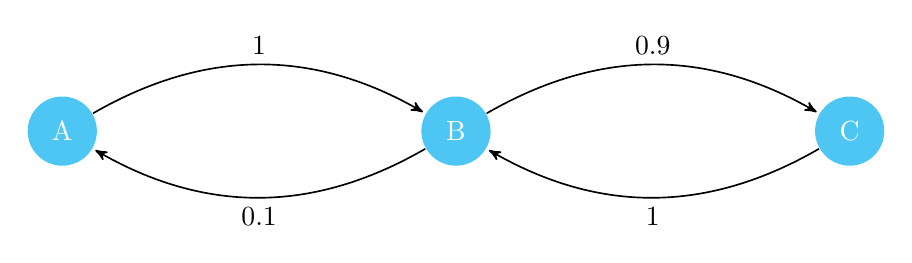
\begin{tikzpicture}[->,>=stealth',shorten >=1pt,auto,node distance=5cm, semithick]
  \tikzstyle{every state}=[fill=cyan!70!white,draw=none,text=white]

 \node[state] (A)  {A};
  \node[state] (B) [ right  of=A] {B};
   \node[state] (C) [ right  of=B] {C};
  \path (A) edge    [bend left]      node {1} (B)
           (B) edge    [bend left]      node {0.1} (A)  
                 edge [bend left] node {0.9} (C)
          (C) edge [bend left]       node {1} (B);
\end{tikzpicture}
\end{center}
\caption{State diagram of a Markov chain with periodic states $A$ and $C$.}
\label{fig:periodic}
\end{figure} 
\subitem
This markov chain can be represented by the followiong transition matrix:
$$ \text{Transition Matrix: }
    \begin{pmatrix}
    A & B & C & \ \\
    0 & .1 & 0 & A\\
    1 & 0 & 1 & B\\
    0 & .9 & 0 & C\\
    \end{pmatrix}
$$
Where any entry in any column represents the probabilities of changing to another state (row letter) given the state we are currently in (column letter). If we always start at state A, then our starting position will be represented by the following vector:$
    \begin{pmatrix}
    1 \\
    0 \\
    0 
    \end{pmatrix}
$
If our starting position A occurs at time $i=0$, we can compute the likelihood of any given state at time $i\geq 1$ where $i$ is an integer greater than or equal to one, with the following expression:

$$
    \text{Likelihood of position} = \text{Transition Matrix}^i \times \text{Start Vector} =  \begin{pmatrix}
    0 & .1 & 0 \\
    1 & 0 & 1 \\
    0 & .9 & 0\\
    \end{pmatrix}^i \times \begin{pmatrix}
    1 \\
    0 \\
    0 
    \end{pmatrix}
$$
We can clearly see that if $i$ is odd, we are in state $B$, as we start in $A$, and immediately go to $B$, and every other state we are in state $B$. Likewise, if $i$ is even, we are either in State $A$ (with probability of $10\%$) or State $C$ (with probability of $90\%$). This is intuitive, because since every odd $i$ we are in state $B$, our odds of ending up in state $A$ or $B$ or $C$ on our next $i$ is governed by the middle vector in our transition matrix, which has probability of $10\%$ that we end up in $A$ and probability $90\%$ that we end up in state $C$.

(Please don't dock me for not using the eigendecomposition)\\
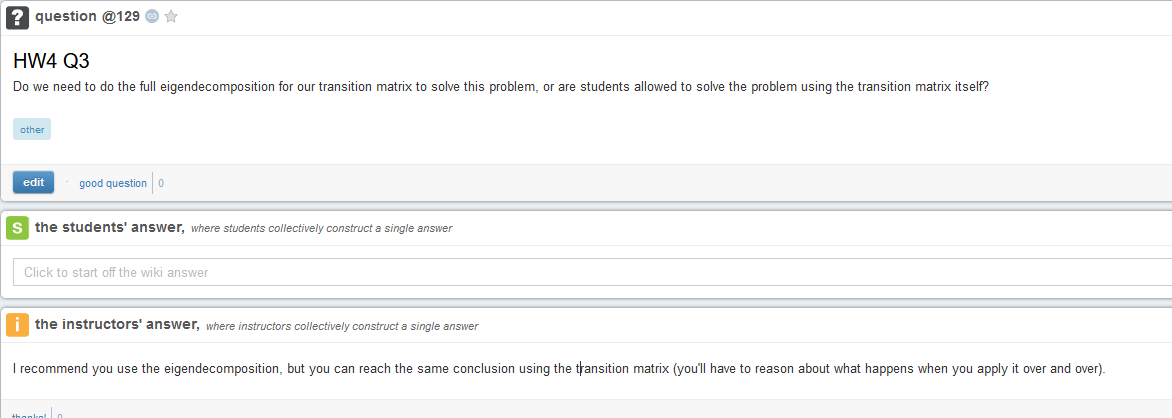
\includegraphics[scale=.5]{answer.png}



\item (Precipitation data) Complete the following code to compute the joint, conditional and marginal pmfs of three random variables representing precipitation in three weather stations:

\url{https://github.com/cfgranda/prob_stats_for_data_science/blob/main/modeling_multivariate_discrete_data/precipitation_EXERCISE.ipynb}

Report the matrices representing any joint, conditional or marginal pmfs with two arguments. Provide the plots generated for the conditional and marginal pmfs with one argument.
\subitem
\textbf{Matrices generated:}\\

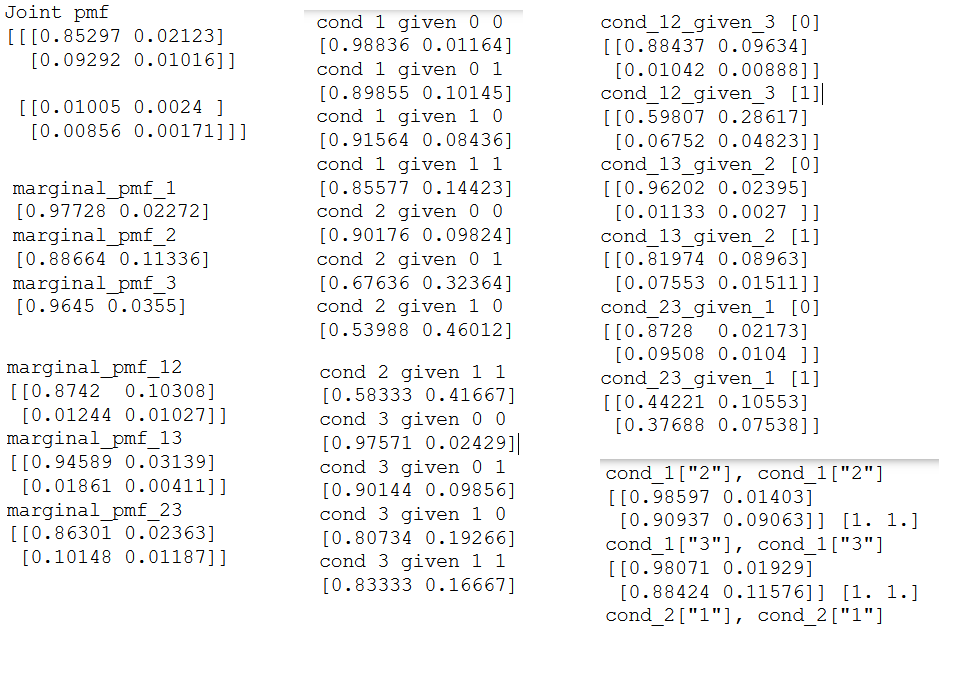
\includegraphics[scale=.7]{hw4 1002 matrices.png}

\textbf{Plots generated:}\\

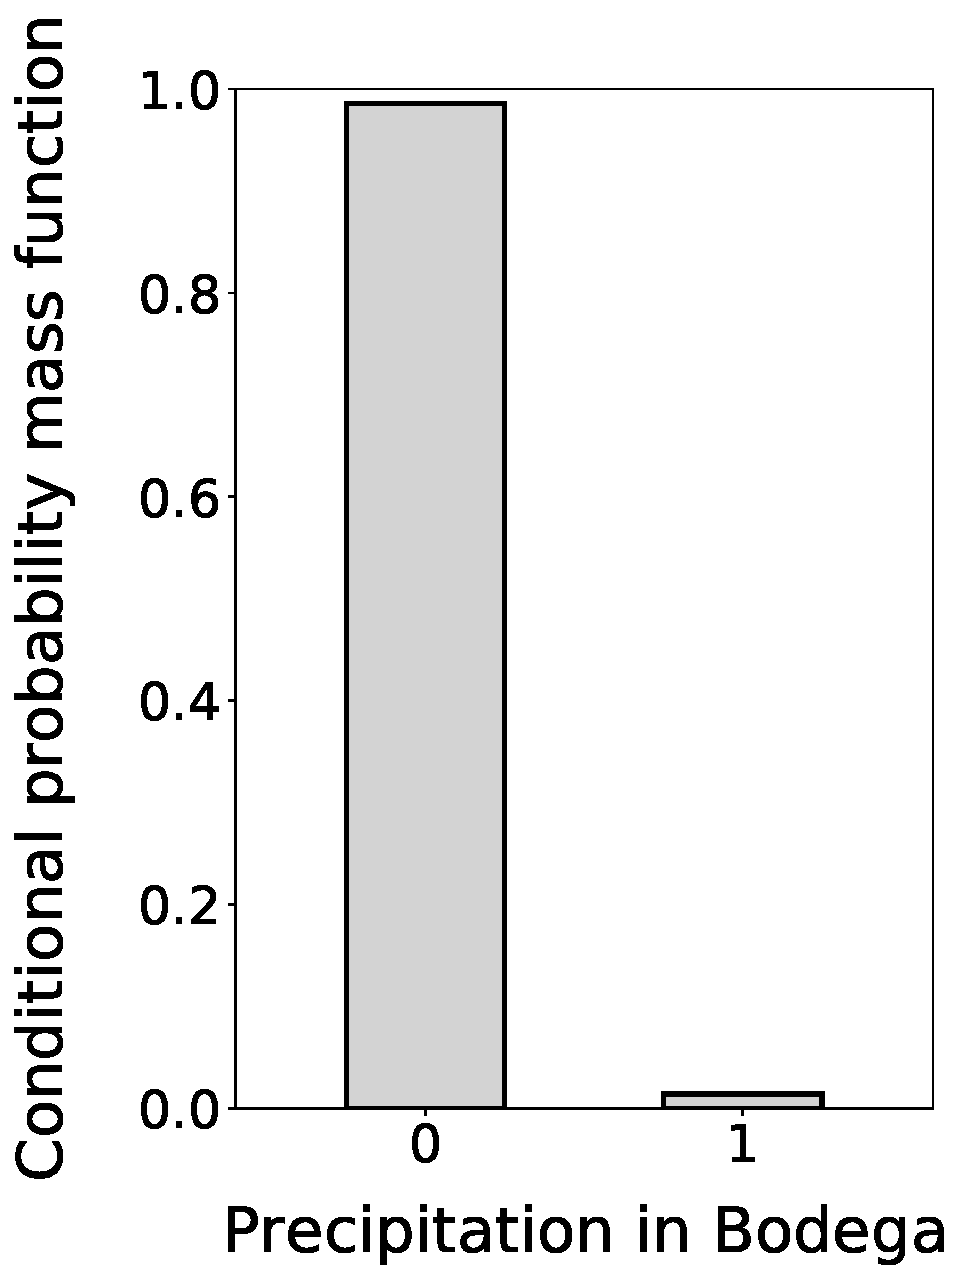
\includegraphics[scale=.5]{precipitation_cond_pmf_1_given_2eq0.pdf}
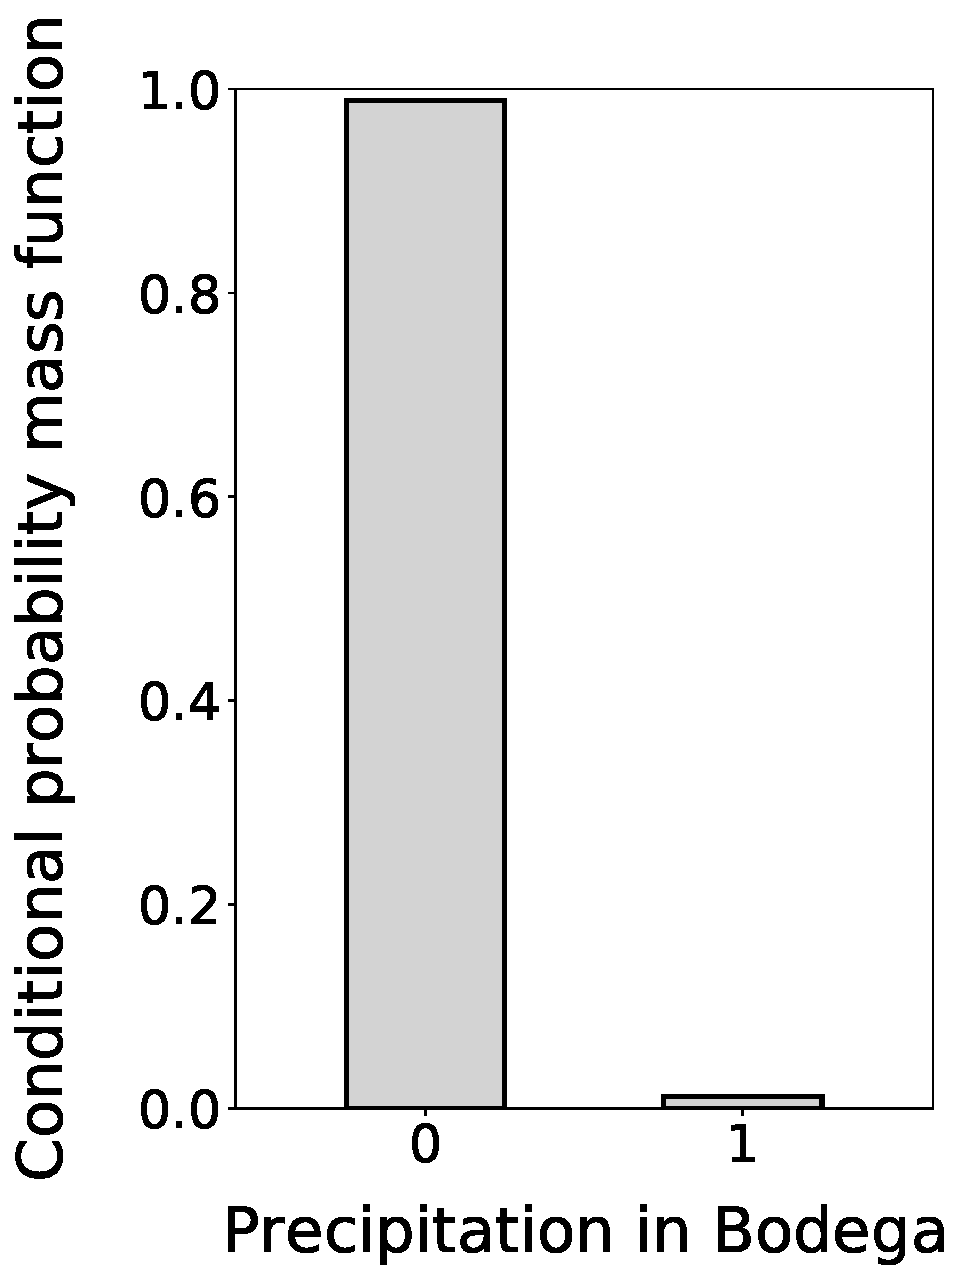
\includegraphics[scale=.5]{precipitation_cond_pmf_1_given_2eq0_3eq0.pdf}
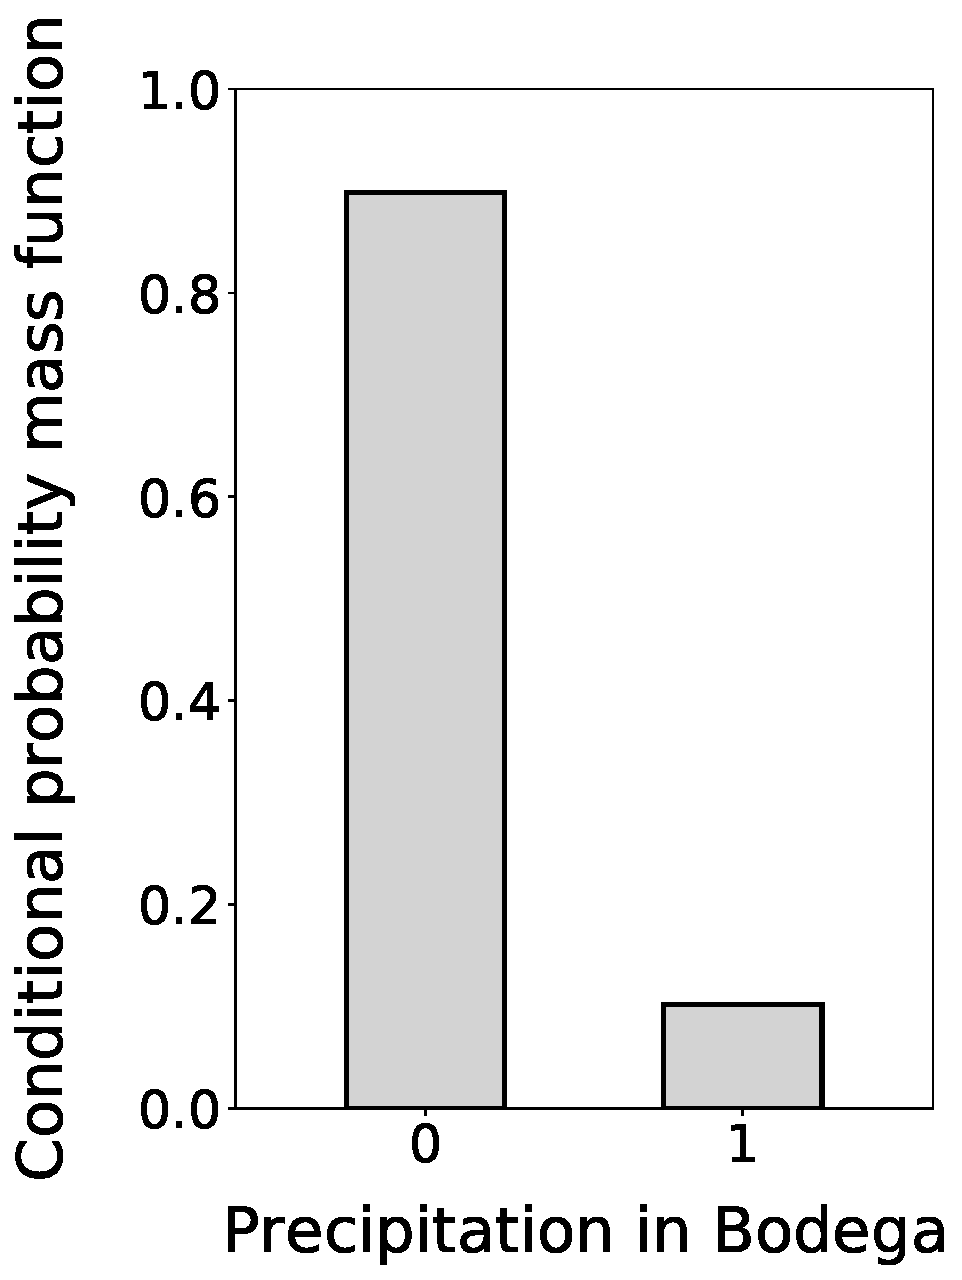
\includegraphics[scale=.5]{precipitation_cond_pmf_1_given_2eq0_3eq1.pdf}
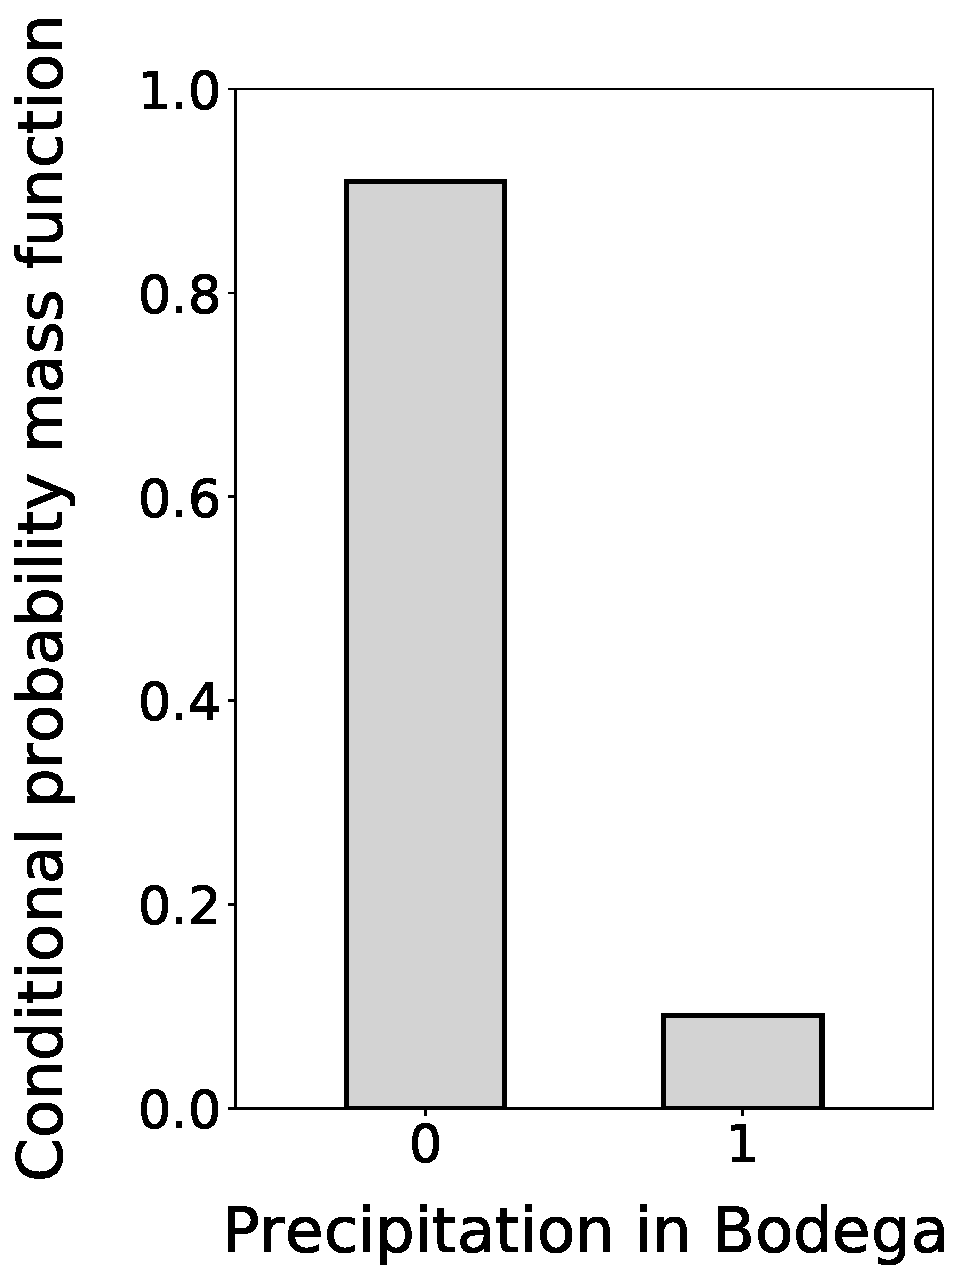
\includegraphics[scale=.5]{precipitation_cond_pmf_1_given_2eq1.pdf}
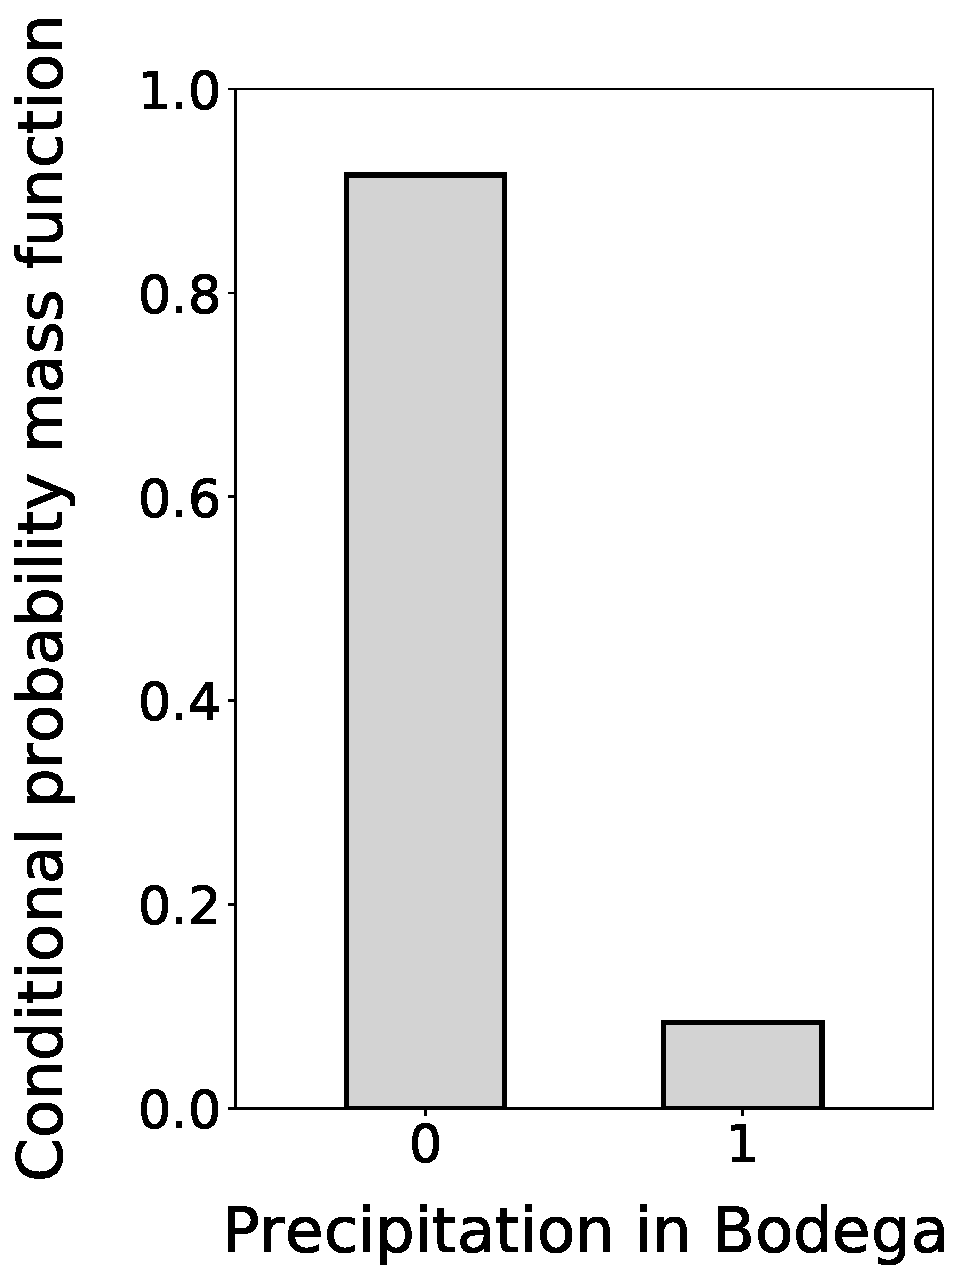
\includegraphics[scale=.5]{precipitation_cond_pmf_1_given_2eq1_3eq0.pdf}
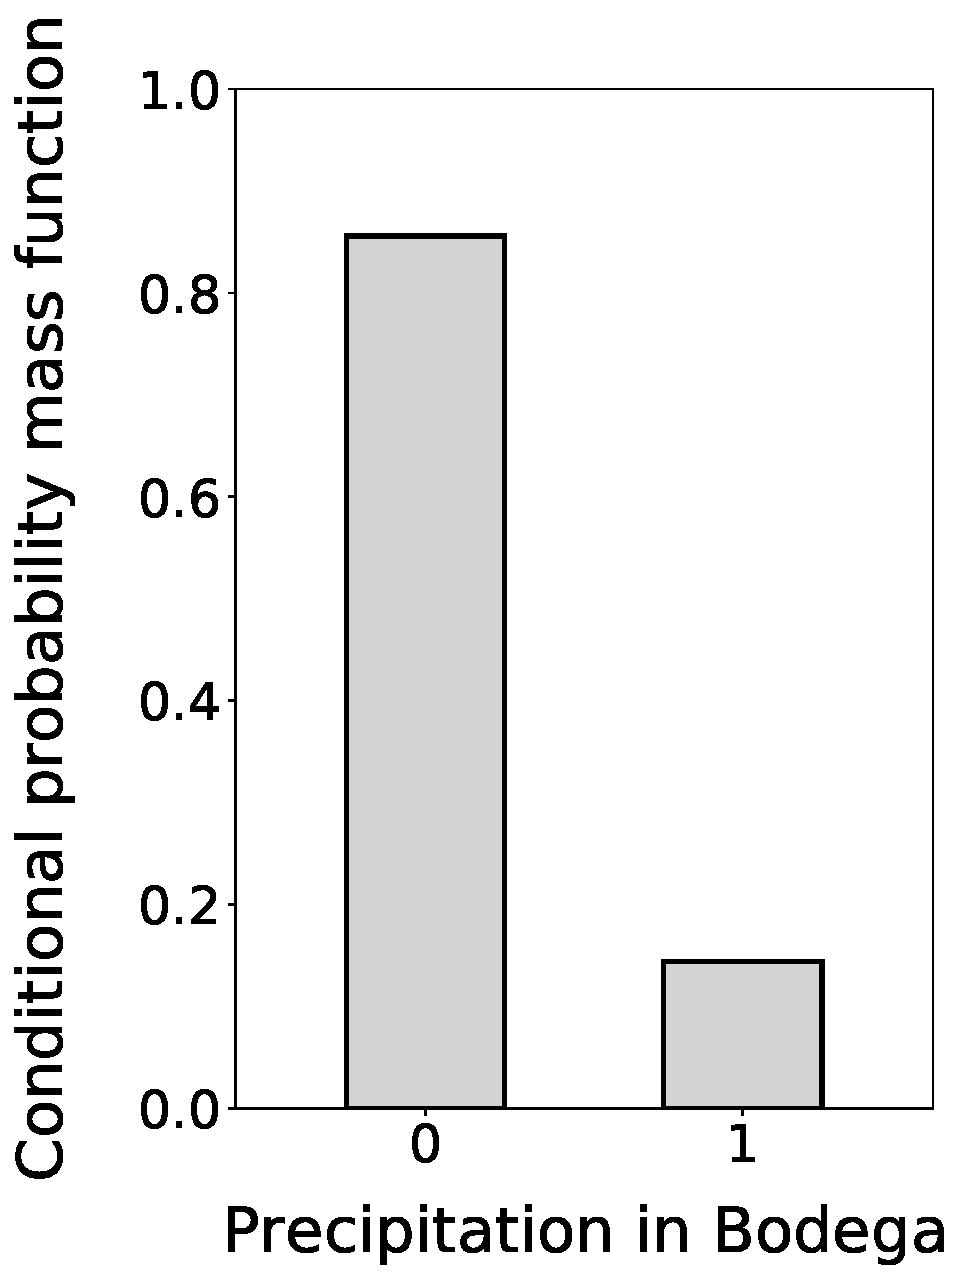
\includegraphics[scale=.5]{precipitation_cond_pmf_1_given_2eq1_3eq1.pdf}
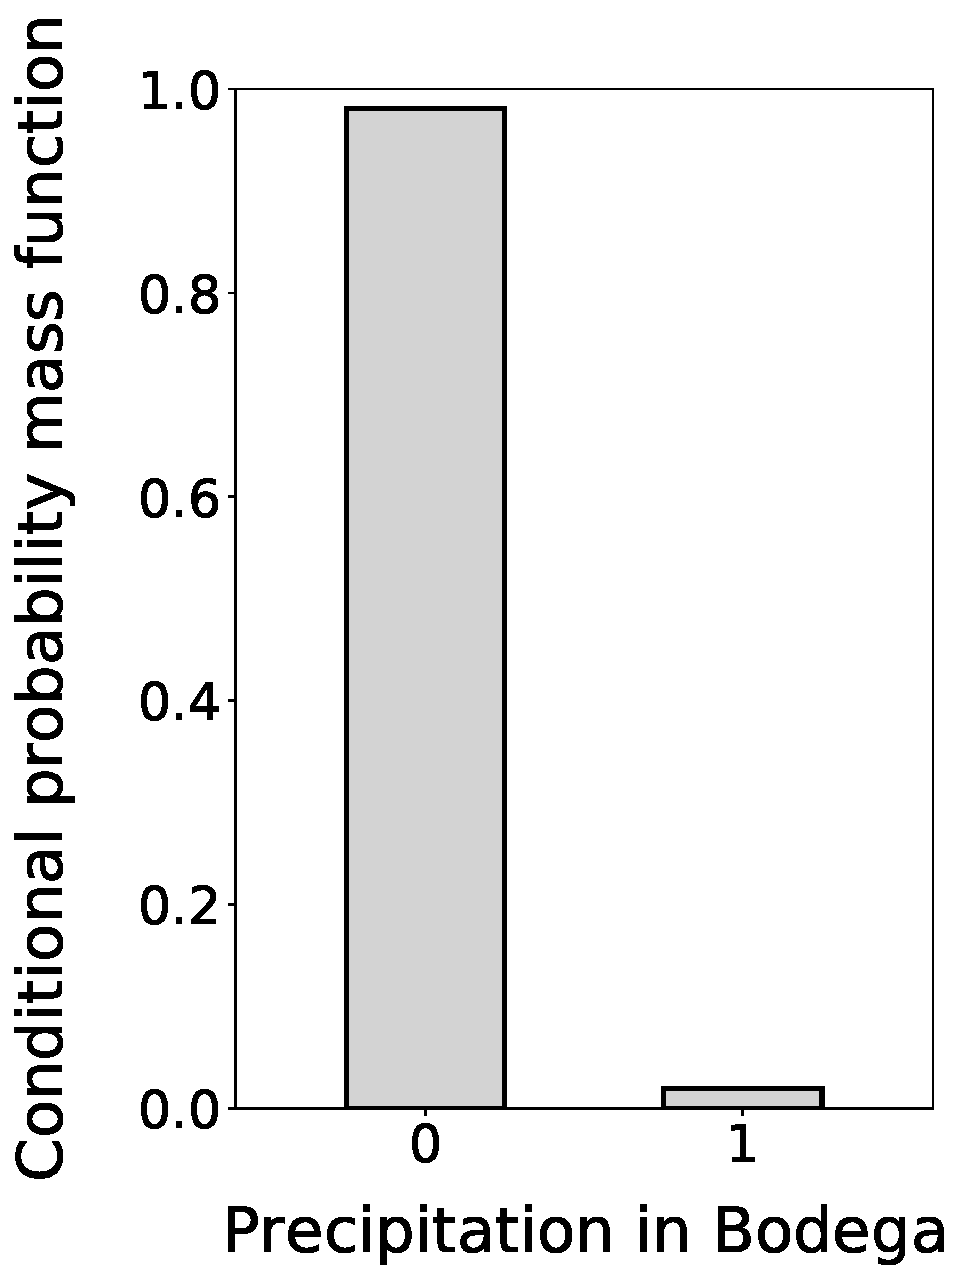
\includegraphics[scale=.5]{precipitation_cond_pmf_1_given_3eq0.pdf}
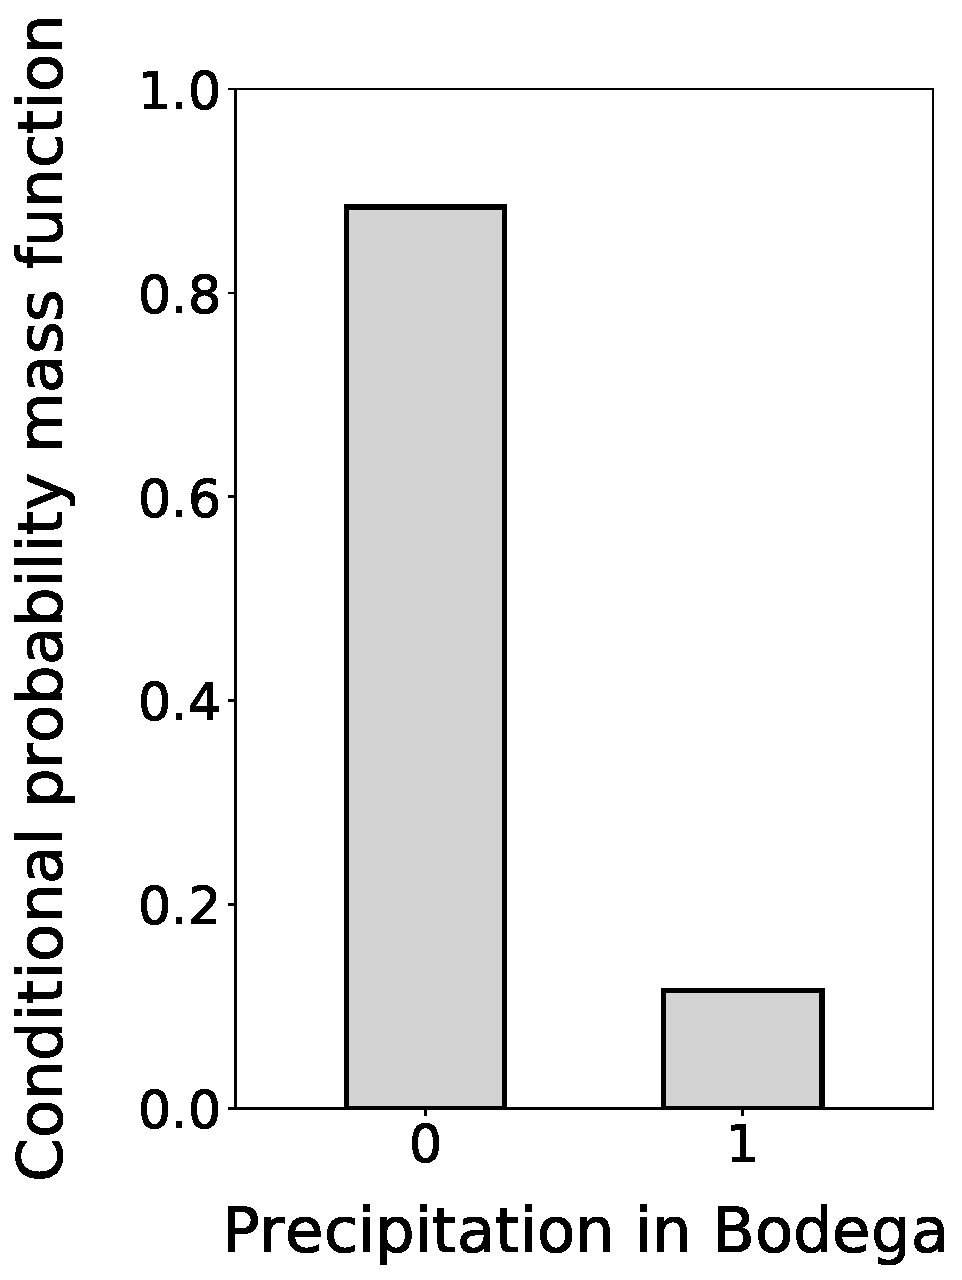
\includegraphics[scale=.5]{precipitation_cond_pmf_1_given_3eq1.pdf}
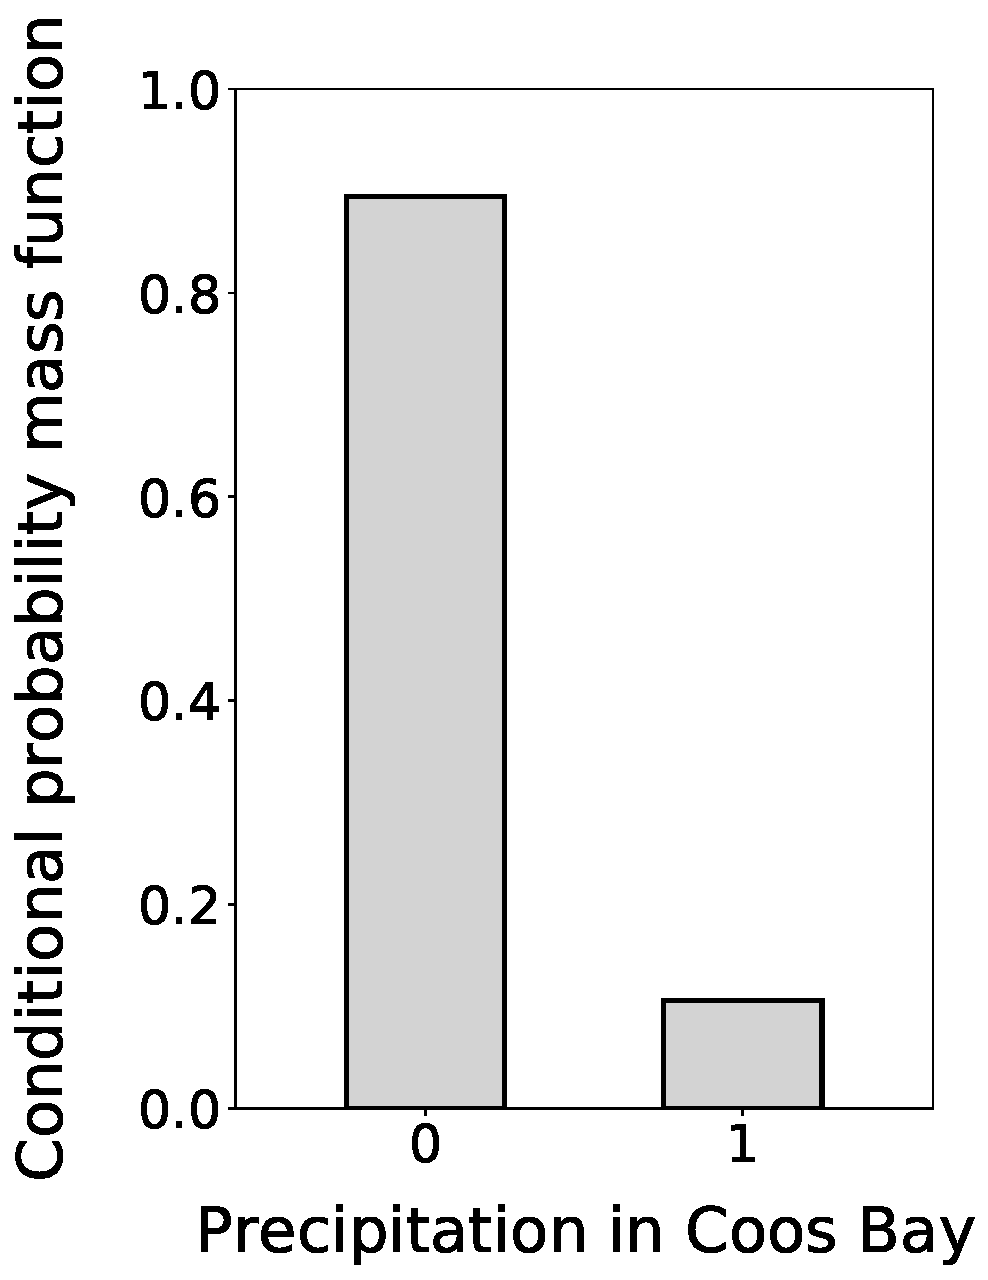
\includegraphics[scale=.5]{precipitation_cond_pmf_2_given_1eq0.pdf}
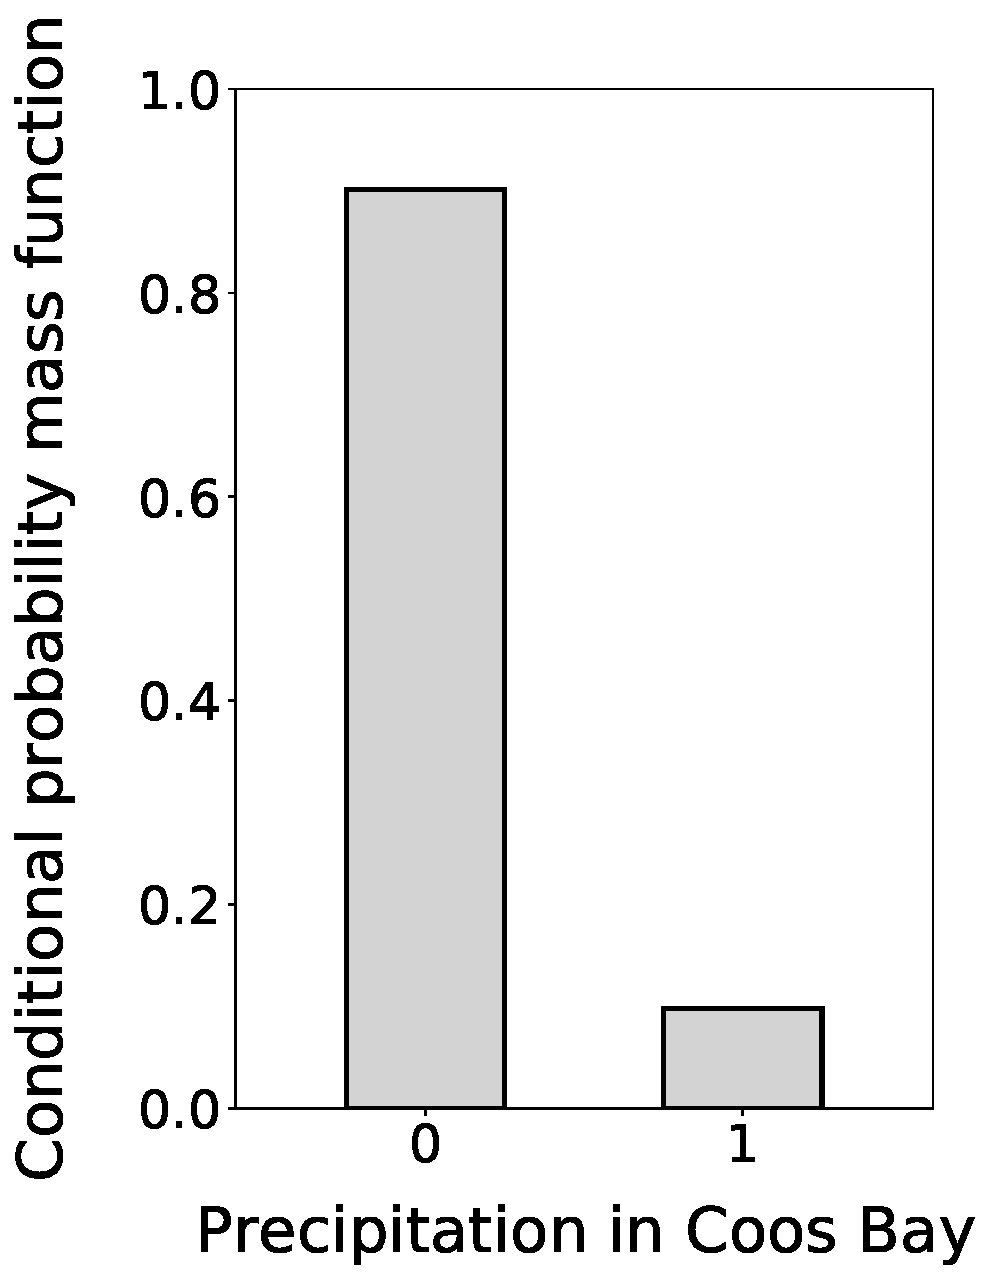
\includegraphics[scale=.5]{precipitation_cond_pmf_2_given_1eq0_3eq0.pdf}
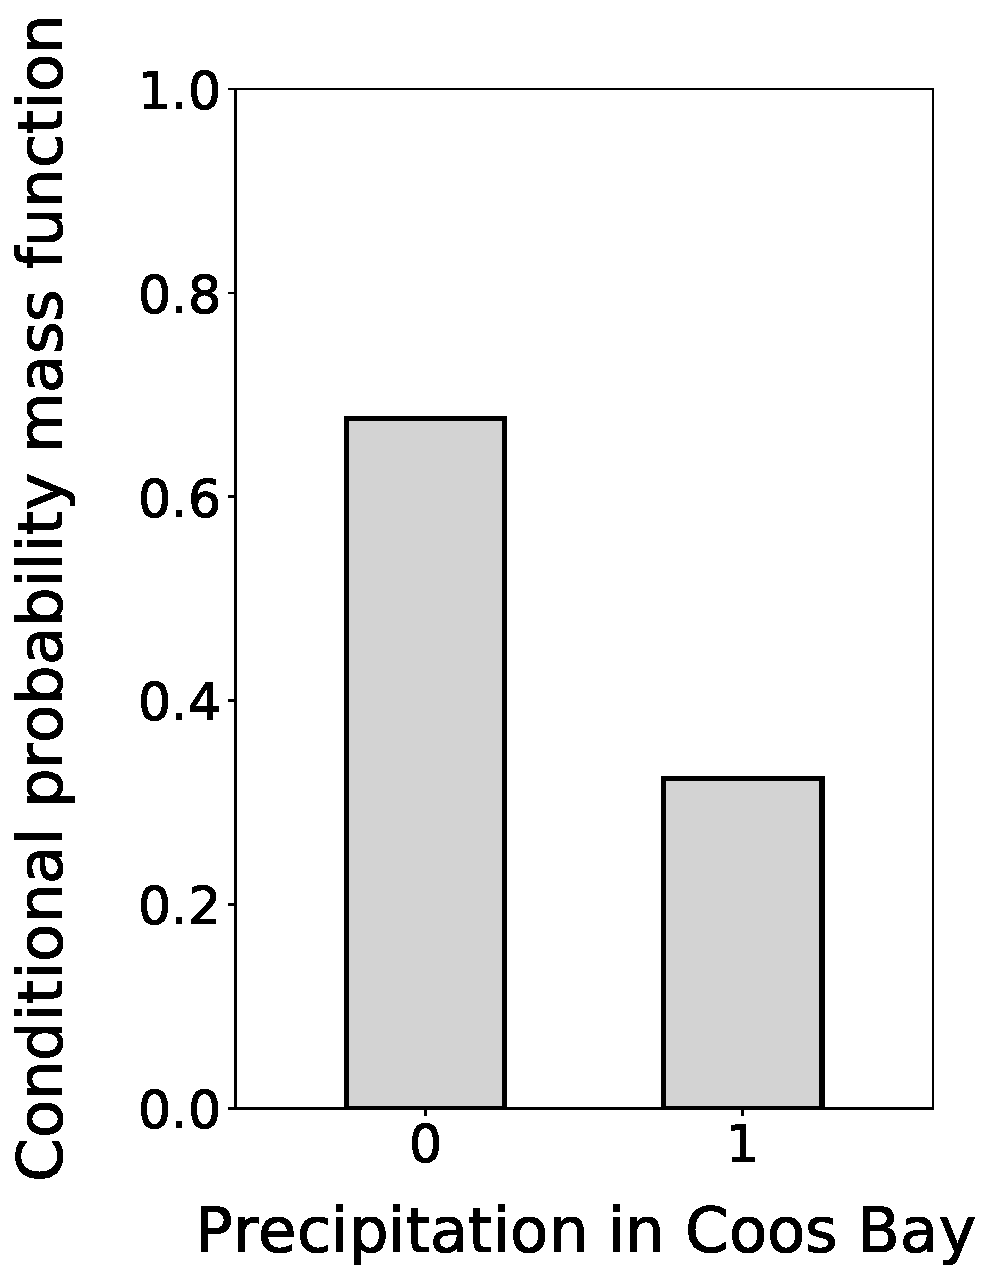
\includegraphics[scale=.5]{precipitation_cond_pmf_2_given_1eq0_3eq1.pdf}
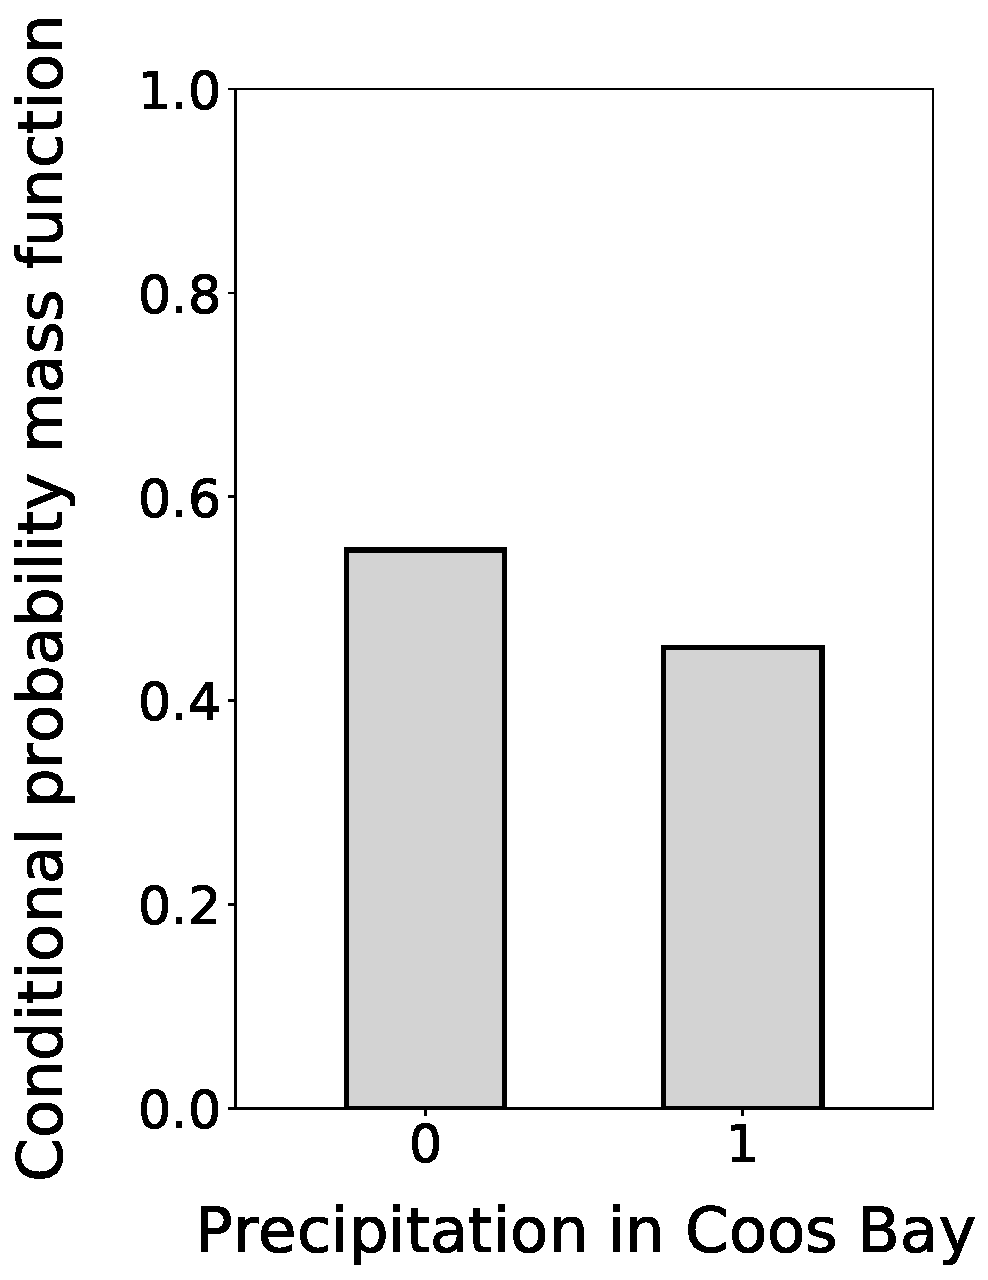
\includegraphics[scale=.5]{precipitation_cond_pmf_2_given_1eq1.pdf}
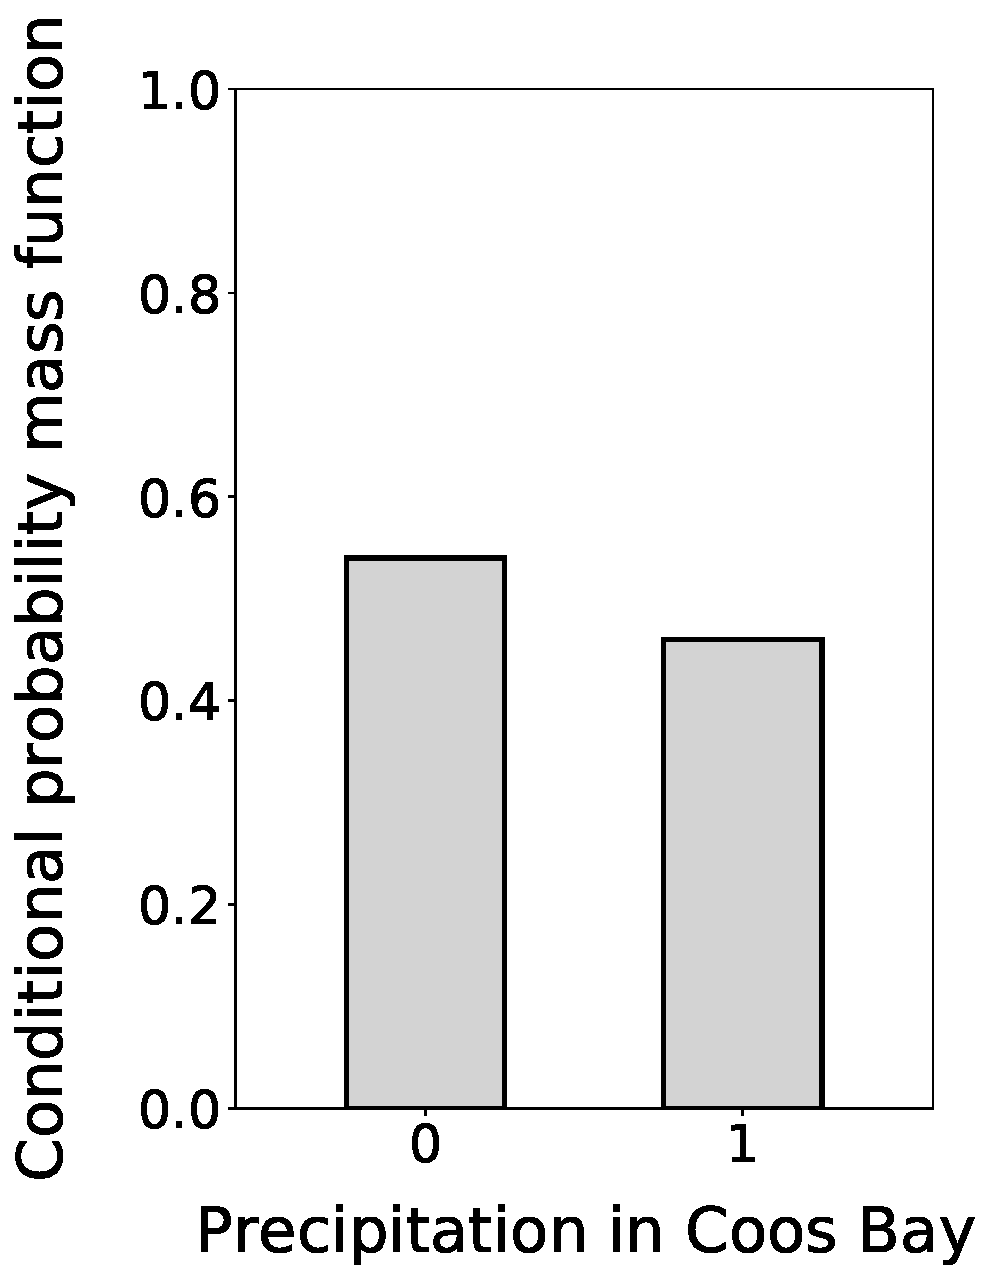
\includegraphics[scale=.5]{precipitation_cond_pmf_2_given_1eq1_3eq0.pdf}
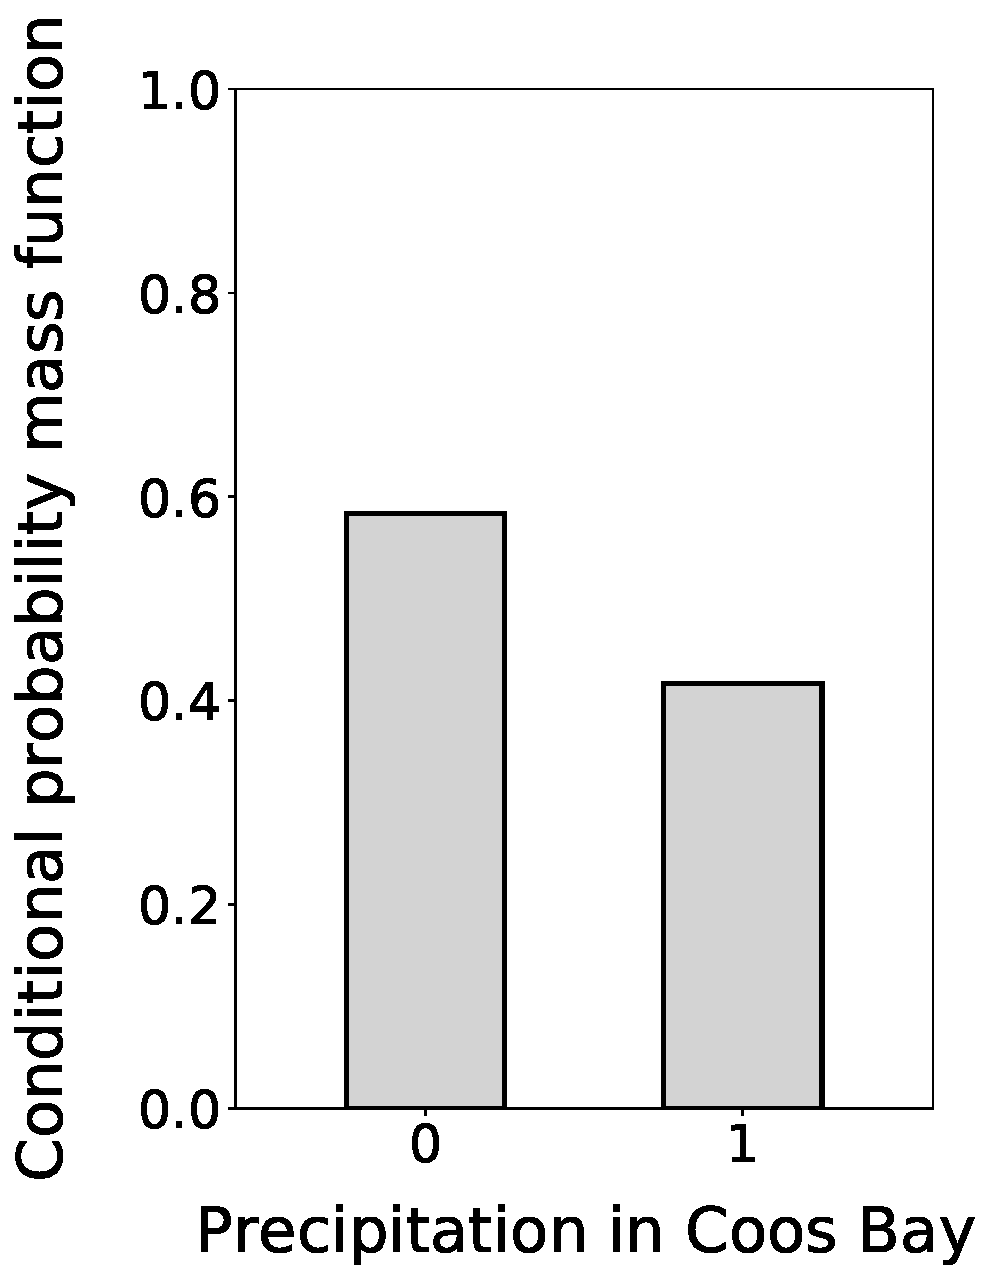
\includegraphics[scale=.5]{precipitation_cond_pmf_2_given_1eq1_3eq1.pdf}
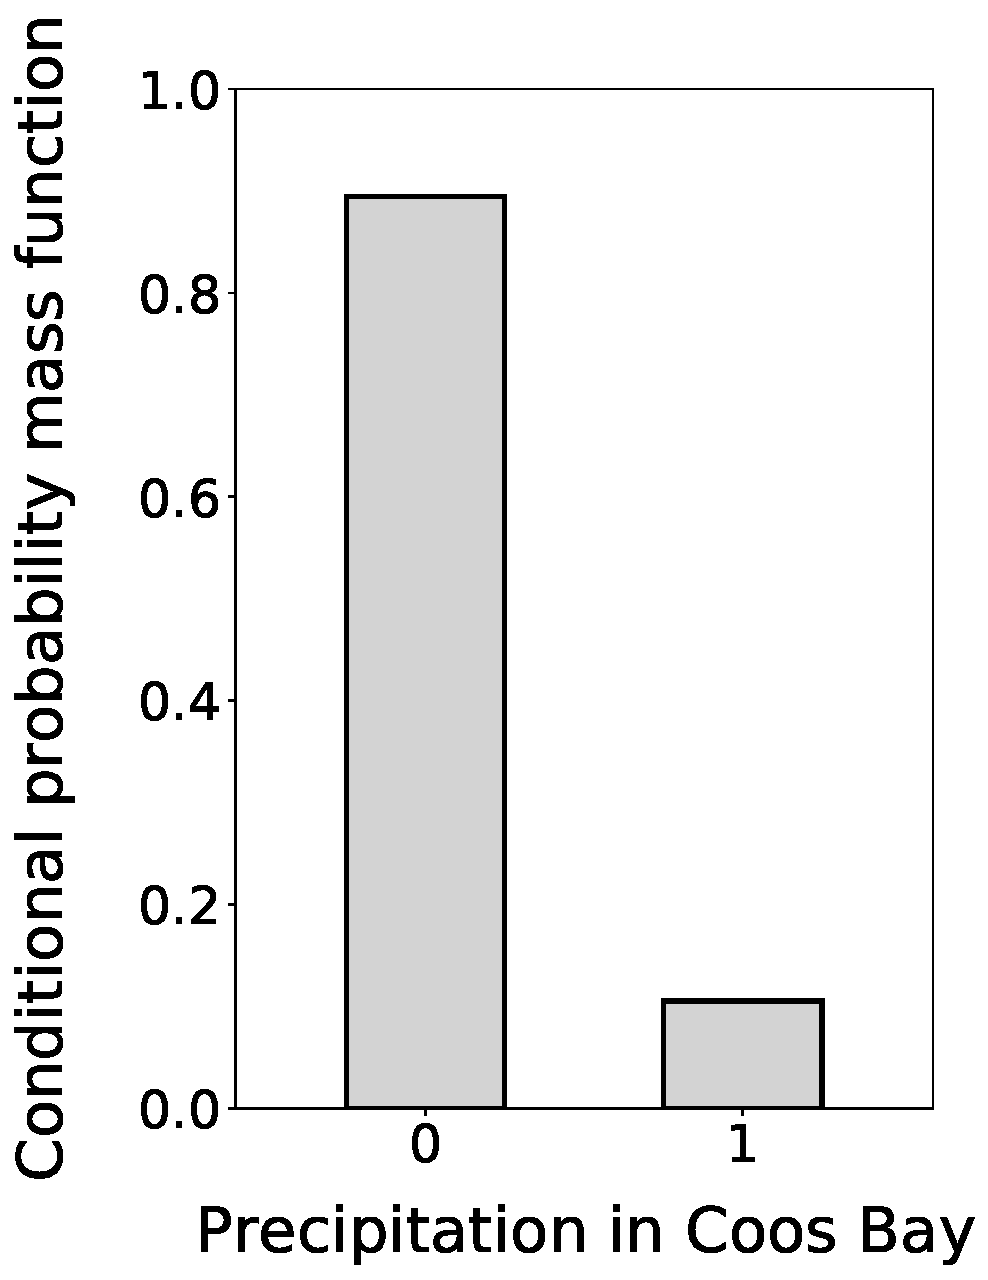
\includegraphics[scale=.5]{precipitation_cond_pmf_2_given_3eq0.pdf}
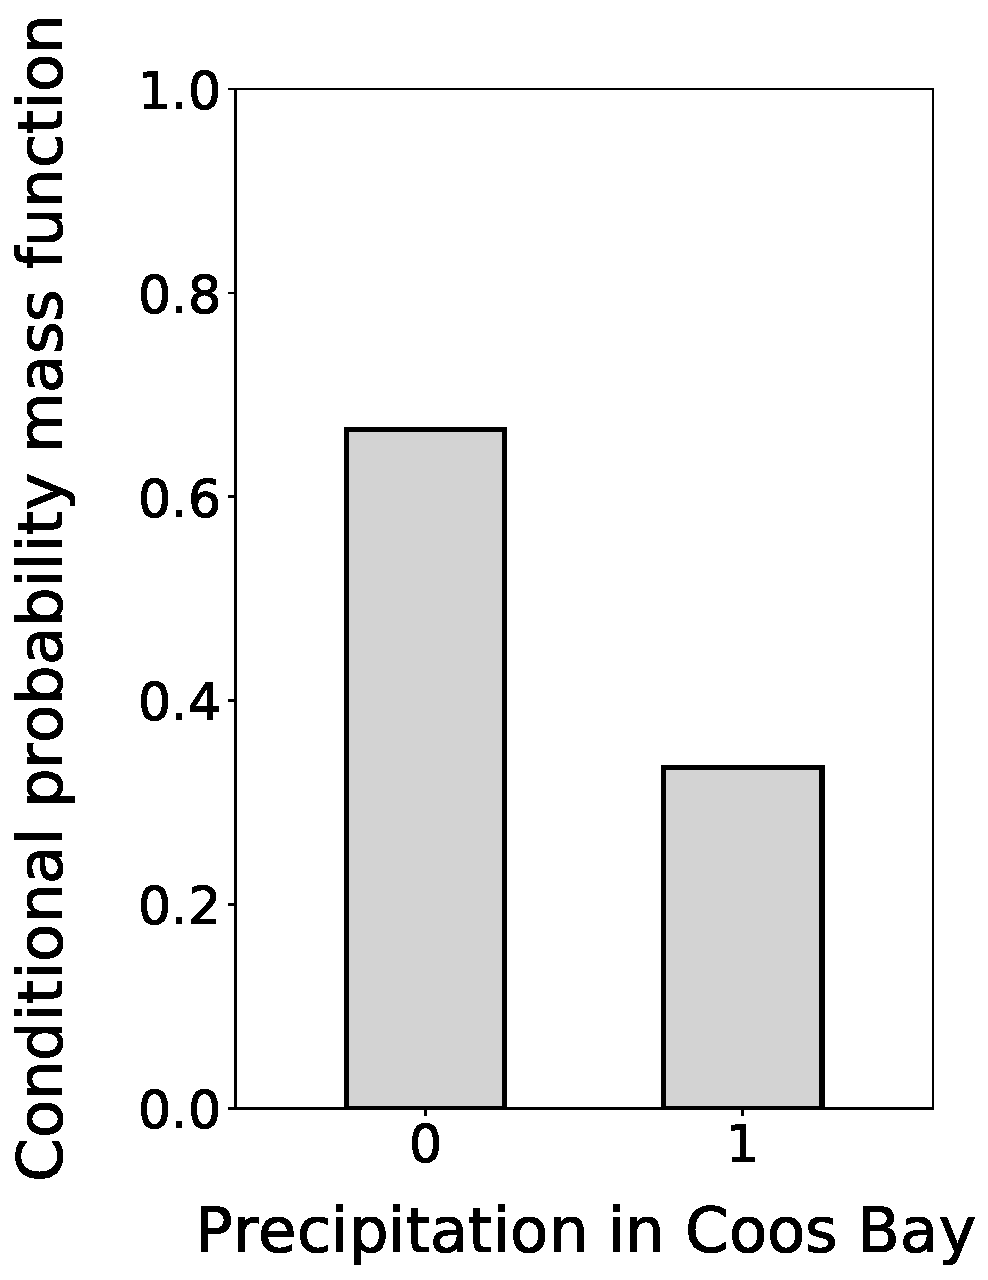
\includegraphics[scale=.5]{precipitation_cond_pmf_2_given_3eq1.pdf}
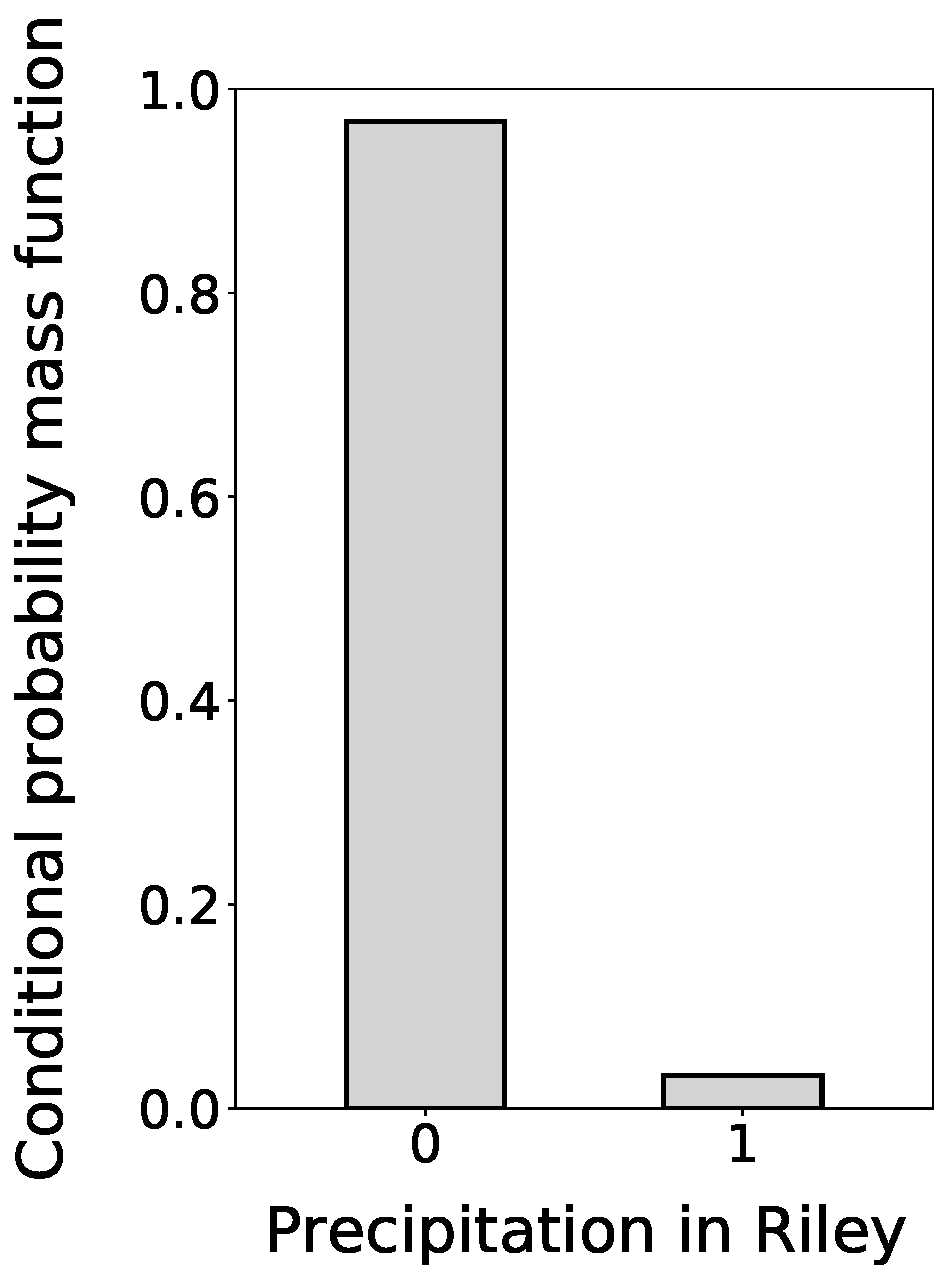
\includegraphics[scale=.5]{precipitation_cond_pmf_3_given_1eq0.pdf}
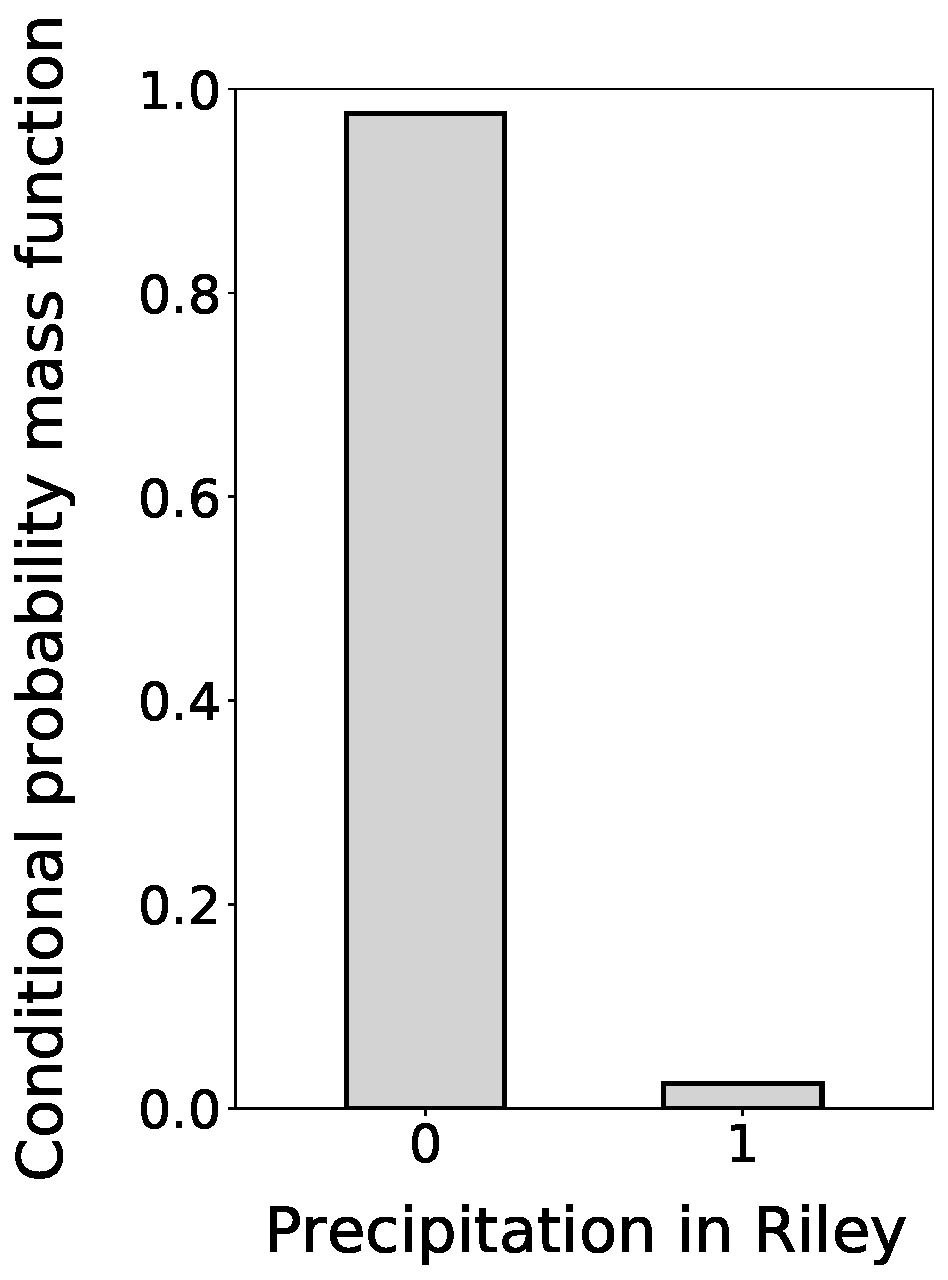
\includegraphics[scale=.5]{precipitation_cond_pmf_3_given_1eq0_2eq0.pdf}
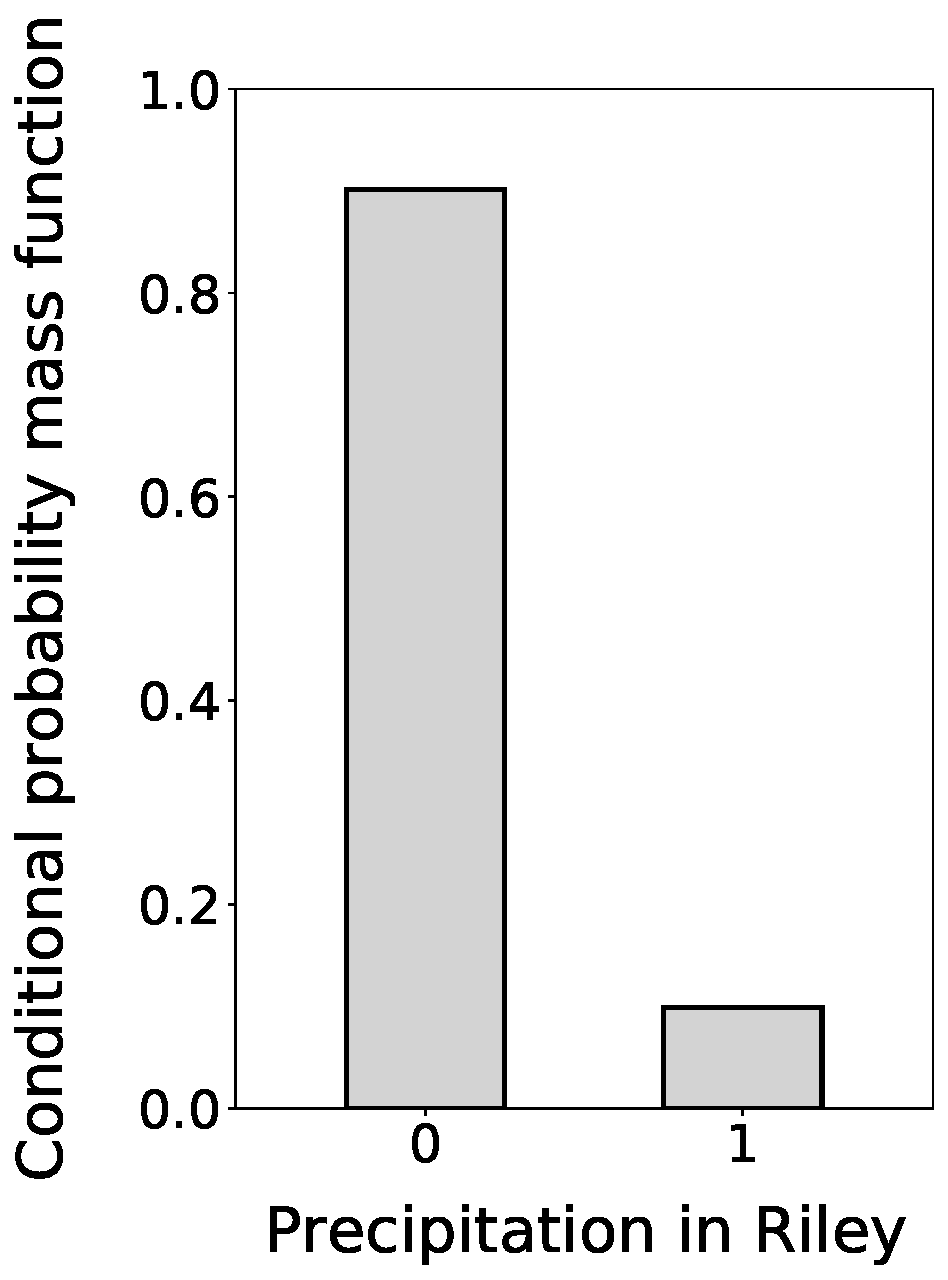
\includegraphics[scale=.5]{precipitation_cond_pmf_3_given_1eq0_2eq1.pdf}
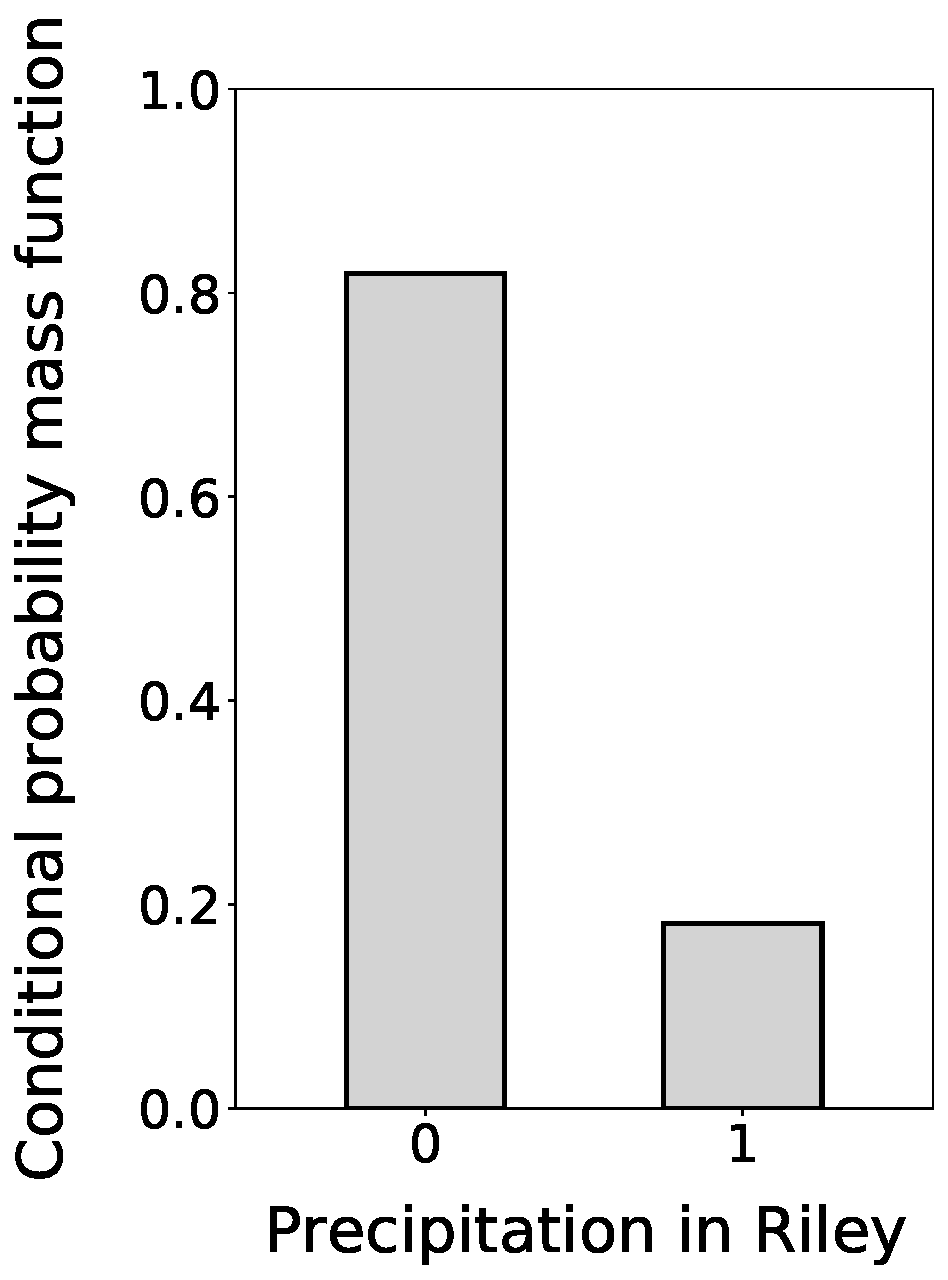
\includegraphics[scale=.5]{precipitation_cond_pmf_3_given_1eq1.pdf}
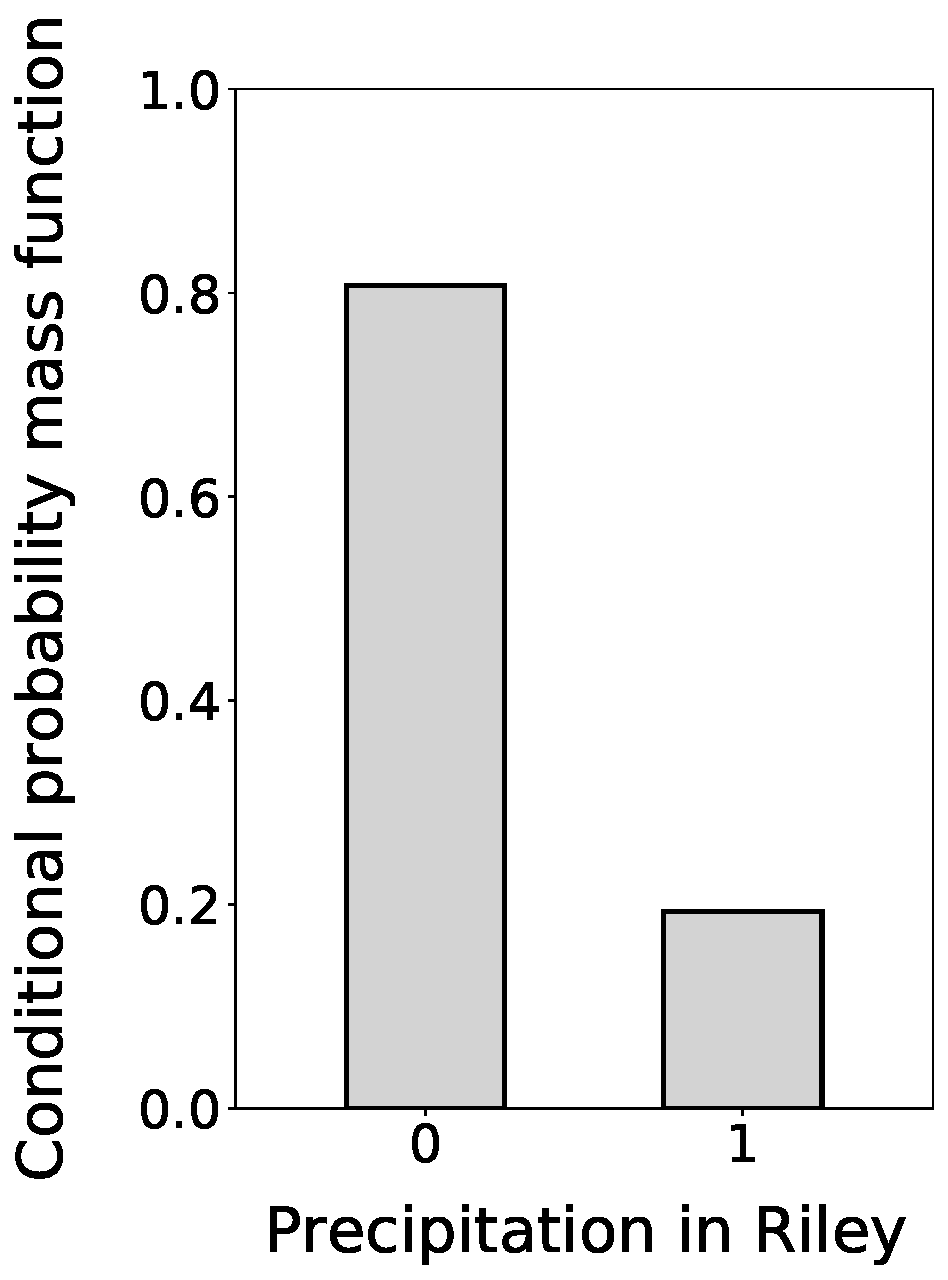
\includegraphics[scale=.5]{precipitation_cond_pmf_3_given_1eq1_2eq0.pdf}
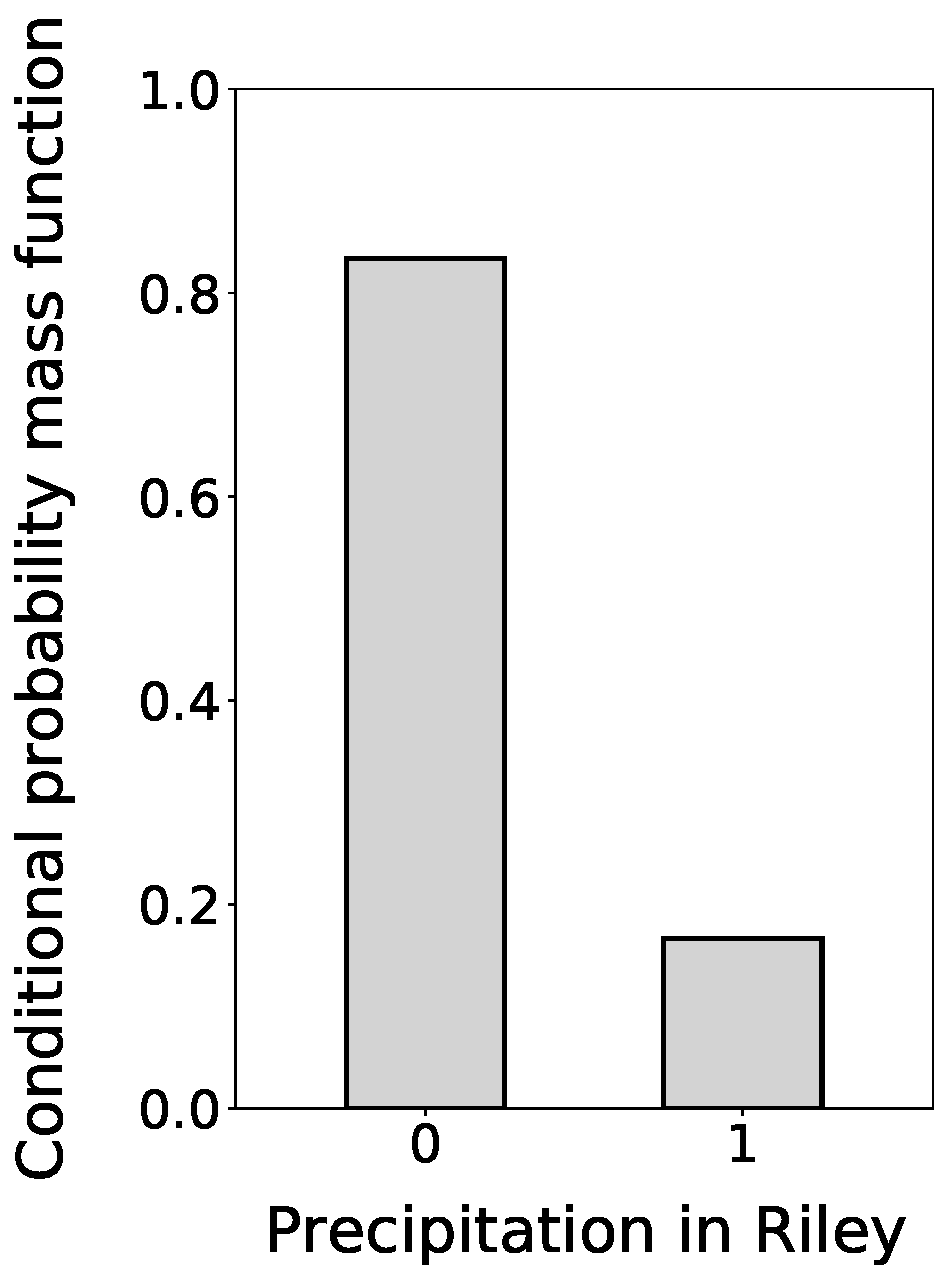
\includegraphics[scale=.5]{precipitation_cond_pmf_3_given_1eq1_2eq1.pdf}
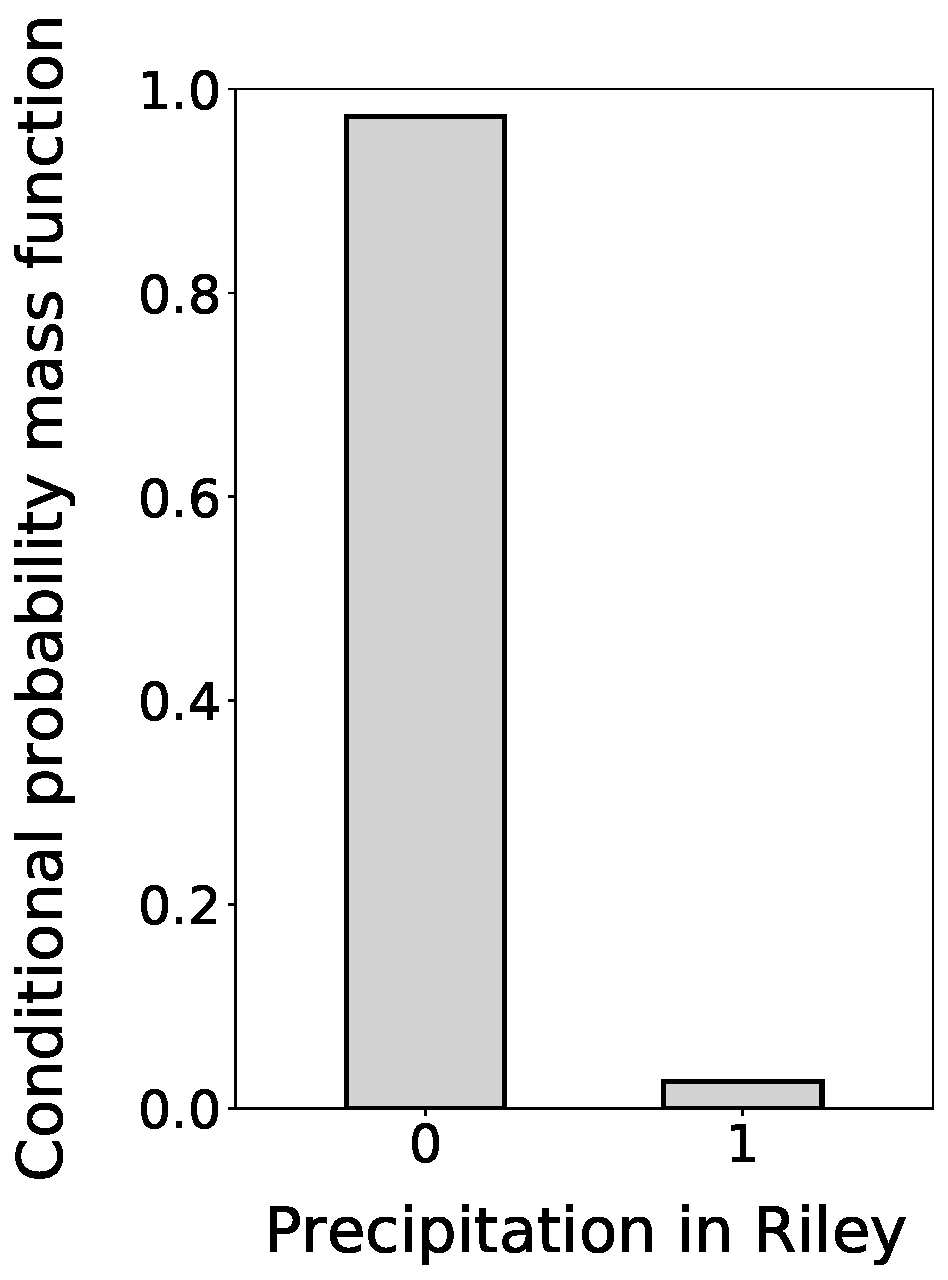
\includegraphics[scale=.5]{precipitation_cond_pmf_3_given_2eq0.pdf}
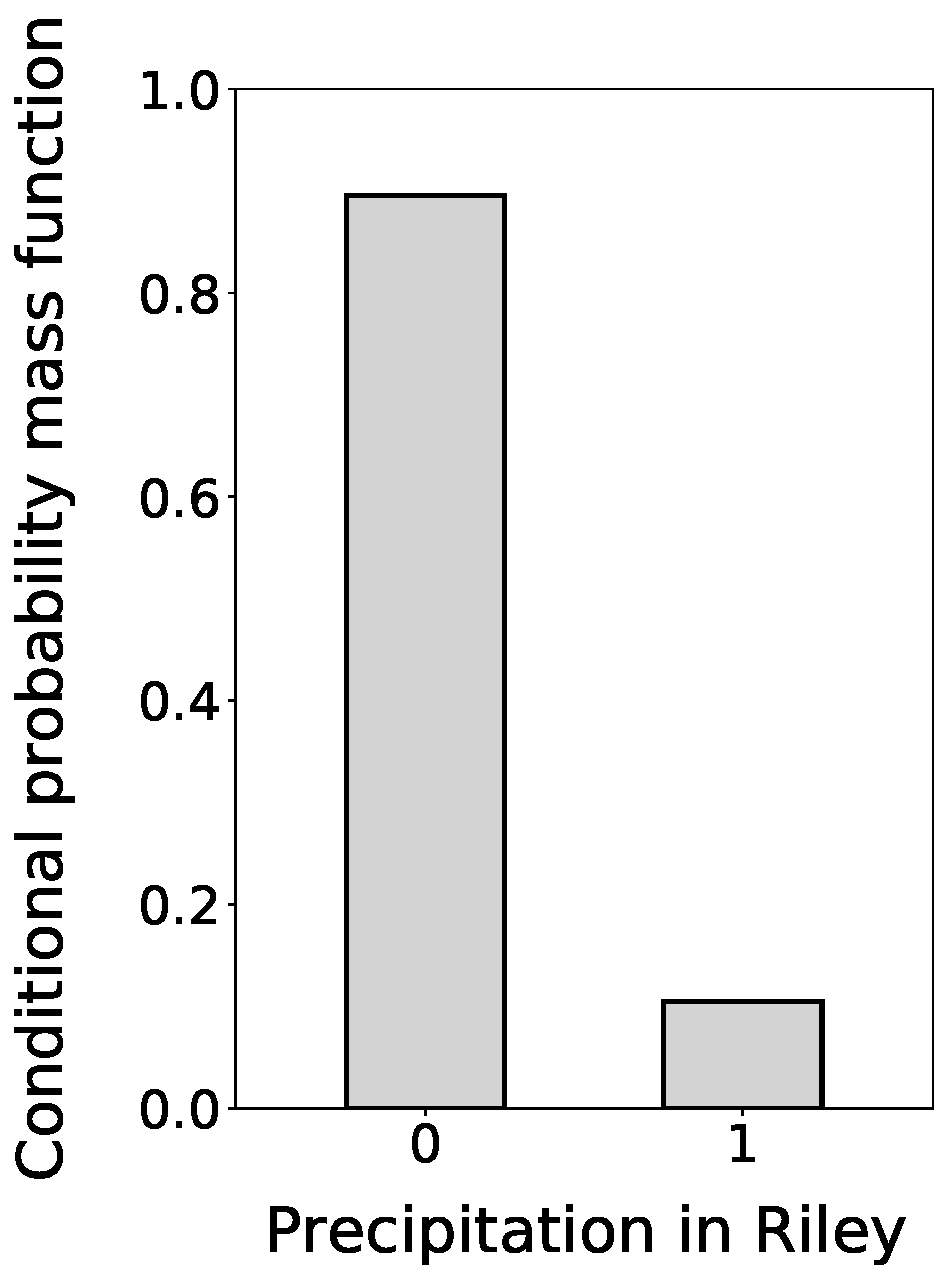
\includegraphics[scale=.5]{precipitation_cond_pmf_3_given_2eq1.pdf}
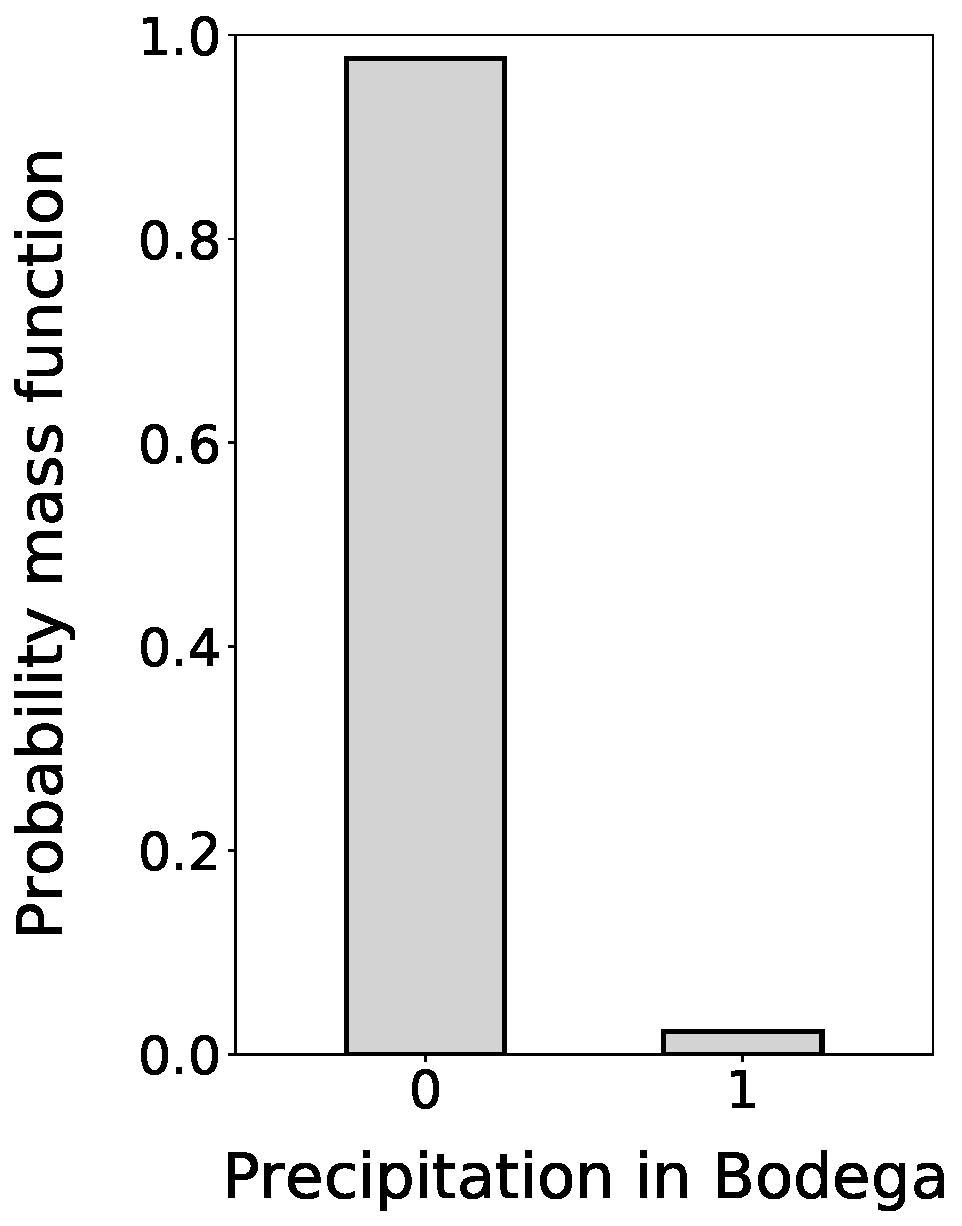
\includegraphics[scale=.5]{precipitation_marginal_pmf_1.pdf}
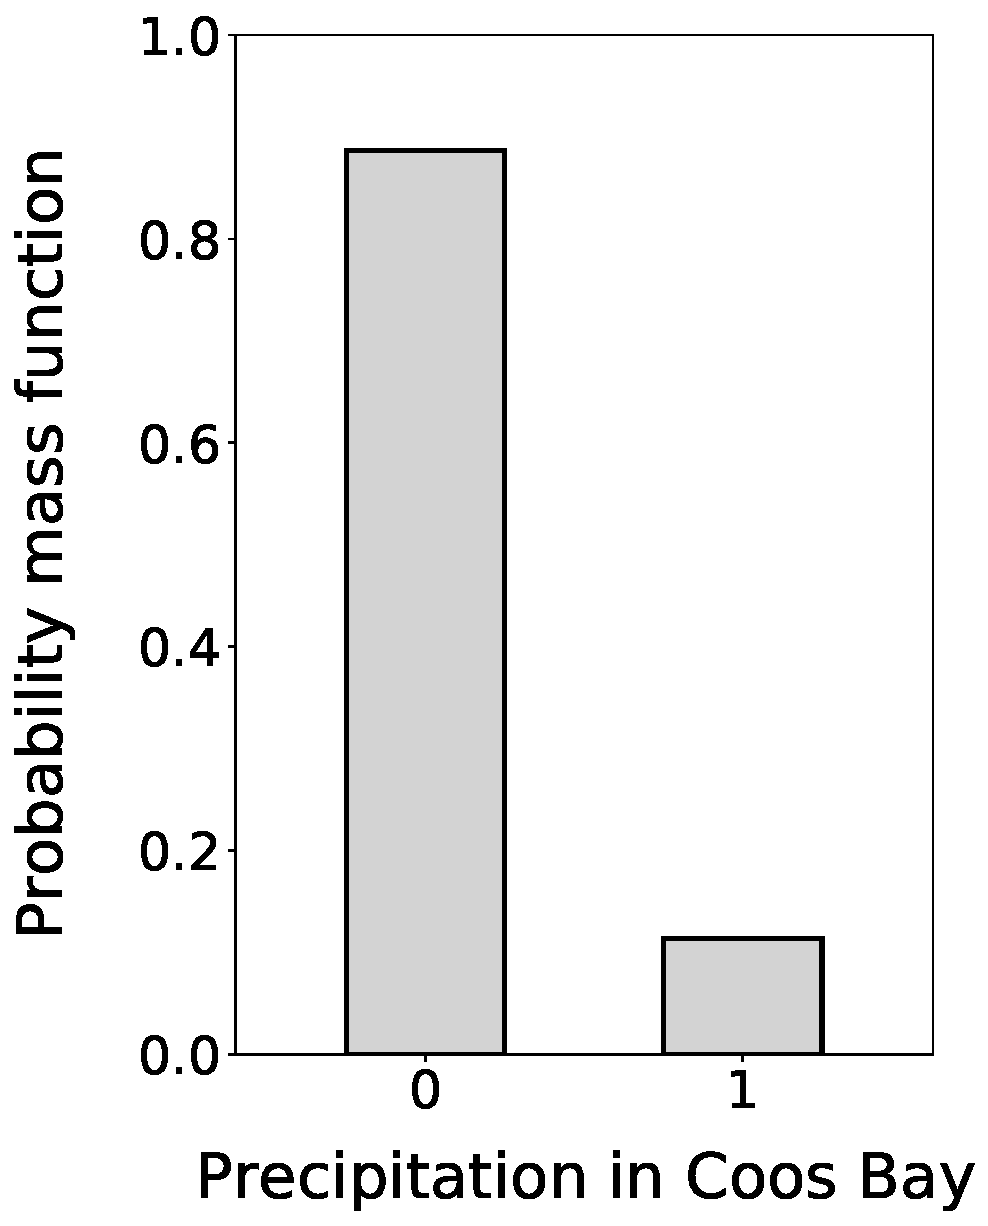
\includegraphics[scale=.5]{precipitation_marginal_pmf_2.pdf}
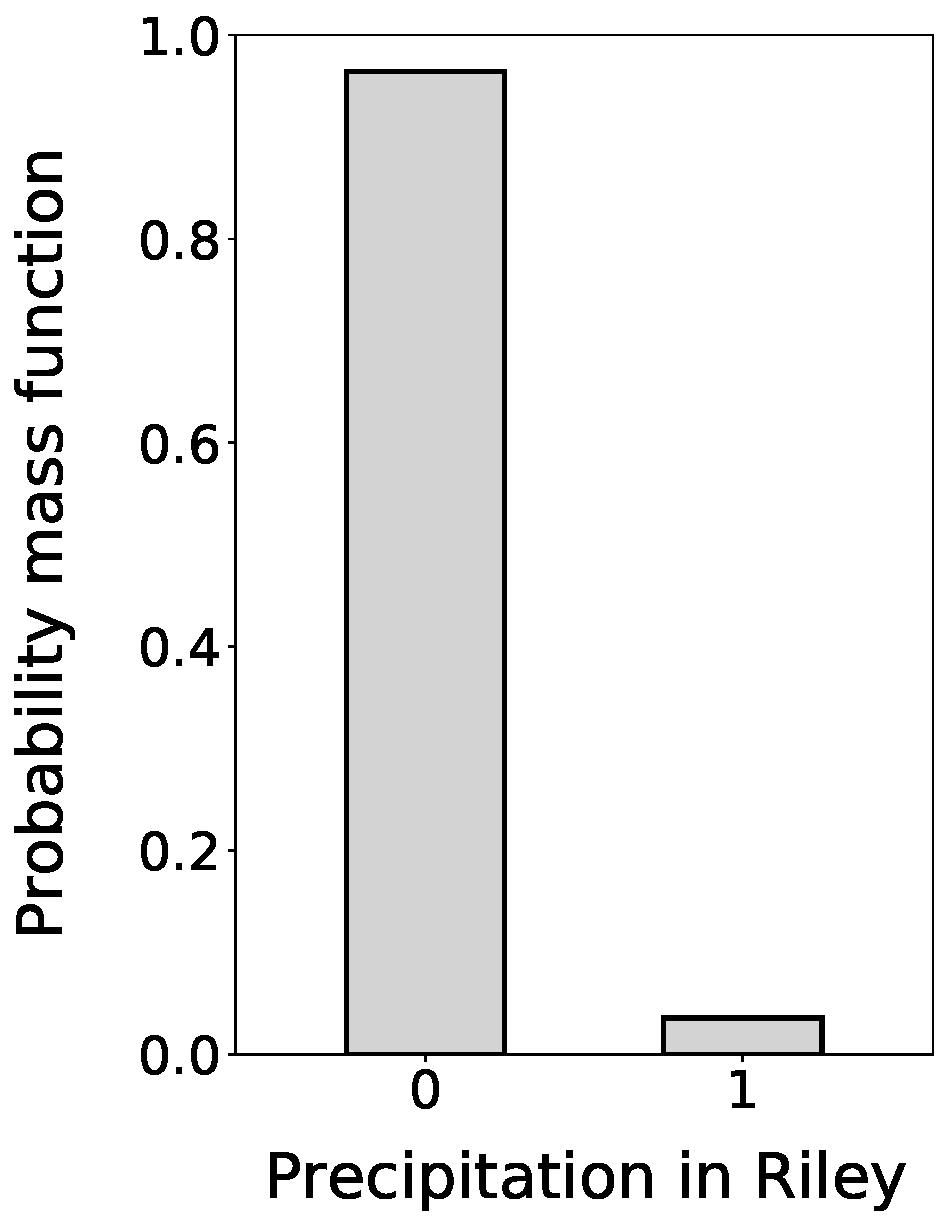
\includegraphics[scale=.5]{precipitation_marginal_pmf_3.pdf}


\end{enumerate}
\end{document}
